% paper.tex
% 9/5/2013 jichi
% Also note that the "draftcls" or "draftclsnofoot", not "draft", option
% should be used if it is desired that the figures are to be displayed in
% draft mode.

%\documentclass[10pt,onecolumn,draftcls,conference]{IEEEtran}
%\documentclass[conference]{IEEEtran}
%\documentclass[preprint]{style/sigplanconf_fixed}
%\documentclass{style/sig-alternate}
%\documentclass[pageno]{style/jpaper}
\documentclass[10pt,doublecolumn,conference]{IEEEtran}

%replace XXX with the submission number you are given from the ASPLOS submission site.
%\newcommand{\asplossubmissionnumber}{267}

% Include my styles
\usepackage{paper}
\usepackage{color}

%\renewcommand{\baselinestretch}{0.99}
\newcommand{\todo}[1]{\textcolor{red}{#1}}

\begin{document}

%
% paper title
%
\title{Overlapping Communication With Computation in MPI Applications}

\author{Jichi Guo$^\dag$, Qing Yi$^\dag$, Jiayuan Meng$^\ddag$, Junchao Zhang$^\ddag$, Pavan Baraji$^\ddag$\\
University of Colorado Colorado Springs$^\dag$\\
Colorado Springs, CO, USA\\
\{jguo2, qyi\}@uccs.edu \\
Argonne National Laboratory$^\ddag$\\
Lemont, IL, USA\\
meng.jiayuan@gmail.com, \{jczhang, baraji\}@anl.gov
}
%\authorinfo{}{}{}

% PLEASE ADD INSTITUTIONS
% make the title area
\maketitle

\begin{abstract}
The performance of distributed memory applications, many of which written in MPI, critically depends on how well the
applications can ameliorate the long latency of remote memory accesses by overlapping them with ongoing computations,
thereby minimizing wait time.
This paper presents a study of the various optimization techniques to enable such overlapping in large MPI applications
and presents a framework towards systematically  enabling a majority of such optimizations.
Our framework first uses analytical performance modeling of the application execution flow,
 combined with application profiling, to automatically
identify potential communication hot spots that may induce long wait time.
%and any nearby computation that may be overlapped with the communication time.
Then, for each communication hot spot,
it searches the call graph to find surrounding loops that includes sufficient local computation
to overlap with the communication.
Finally,  blocking MPI communications are decoupled into non-blocking operations when necessary, and their surrounding loop
transformed to hide the communication latencies behind local computations.
%We use the MPI\_Test operation inserted into the transformed code
%  to dynamically adjust the communication frequency. % jichi: ``progress'' is a terminology to describe the poll-based MPI communication engine
%The execution frequency of MPI\_Test if in loops is tuned for different input data and runtime environment using binary search.
%Finally, modify the workflow.
We evaluated our framework using 7 MPI applications from the \texttt{NAS} Benchmark suite.
Our optimizations are able to attain 3\% to 72\% speedup over the original implementations.
\end{abstract}


\lstdefinelanguage{sklt}{
  morecomment=[s]{/*}{*/},
  morecomment=[l]{//},
  morekeywords={
    dummy,
    def, call, from, import,
    stream, for, forall, switch, case, if, else, return, break, continue,
    st, ld, comp, ilp, blk, block,
    int, long, float, double, char, string,
    for_threads, grid, thread_block, commit,
    comm, send, recv, bcast, barrier, allreduce, sendrecv, all2all, reduce,
  },
}

\lstset{
  language=sklt,
  keywordstyle=\bf,
  %keywordstyle=\em\bfseries,
  basicstyle=\ttfamily\scriptsize,
  numbers=left,
  numberstyle=\tiny,
  stepnumber=2,
  numbersep=3pt,
}

\section{Introduction}
\label{sec:intro}

As computing platforms migrate to clusters of increasingly larger scale of microprocessors,
 applications need to manage the distributed memories of the processors via explicit
message-passing runtimes, for example, MPI, to attain high performance.
The relative latency and bandwidth of the communication network in relation to the compute capacity of processors
are often hard to predict a priori and may change dramatically from one system to the next.
Even on supercomputers comprising homogeneous nodes,
system noise is increasing on each node because of aspects such as power management, deeper memory hierarchies, and sharing of hardware such as caches and network. The ``equal work means equal time" paradigm is no longer relevant on most systems, and load imbalance increasingly becomes the common scenario even on applications that are symmetrically structured.
Consequently, bulk-synchronous communication, where all processes synchronize frequently, is no longer a valid option for high-performance MPI applications.
Application performance is often critically determined by its ability to flexibly overlap communications with local computations,
thereby minimizing wait time.


This paper aims to automatically enable the use of nonblocking latency-hiding techniques to overlap local computation with remote communication in MPI applications, thereby enhancing their overall efficiency and performance portability.
%through a framework that systematically combines analytical performance modeling of the application execution flow and compiler-assisted safety and profitability analysis.
To illustrate the optimization, Figure~\ref{fig:ft_loop} shows the
structure of the NAS FT benchmark~\cite{npb}, which applies fast
Fourier transform (FFT) to a 3D matrix through a loop that interleaves
the computation of scaling the input matrix with a collective
communication of MPI\_Alltoall to exchange data among the
processes. This is then followed by a final transposition of the
resulting matrix.  The clear separation of computation and
communication phases makes the algorithm design easy to implement and
maintain.  Additionally, the communication buffers can be reused
across different loop iterations, saving memory.  However, the
blocking MPI communication requires that all processes wait while the
MPI\_Alltoall operation is in progress.  Consequently, unless the
application is executed on a platform with the fastest network
connections, its performance is likely to suffer because of the
excessive wait time.

\begin{figure}
  \centering
  \begin{subfigure}[b]{0.25\textwidth}
    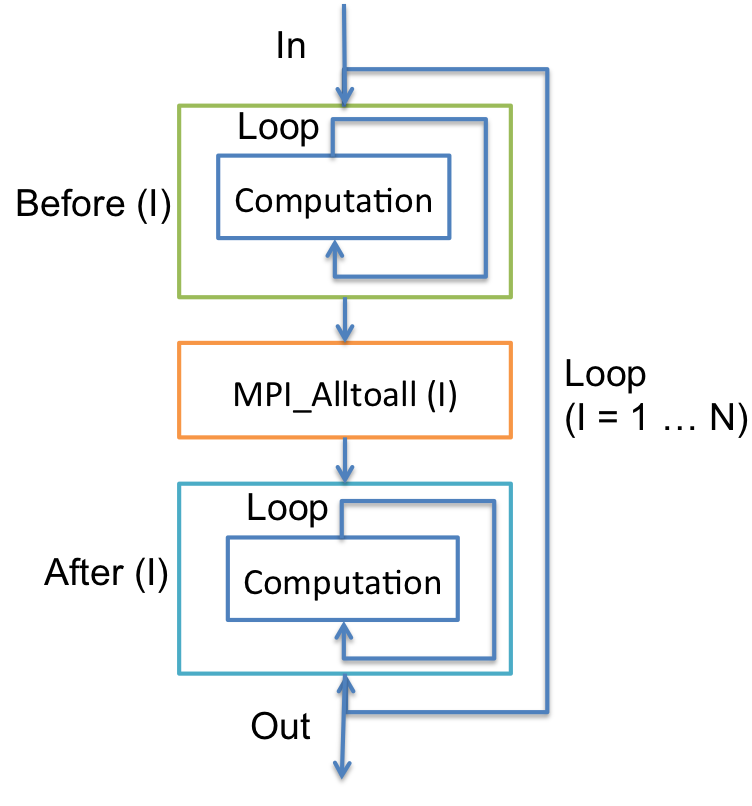
\includegraphics[width=1\textwidth]{fig/ft_loop.png}
    \caption{Before optimization}
    \label{fig:ft_loop}
  \end{subfigure}%
  \begin{subfigure}[b]{0.232\textwidth}
    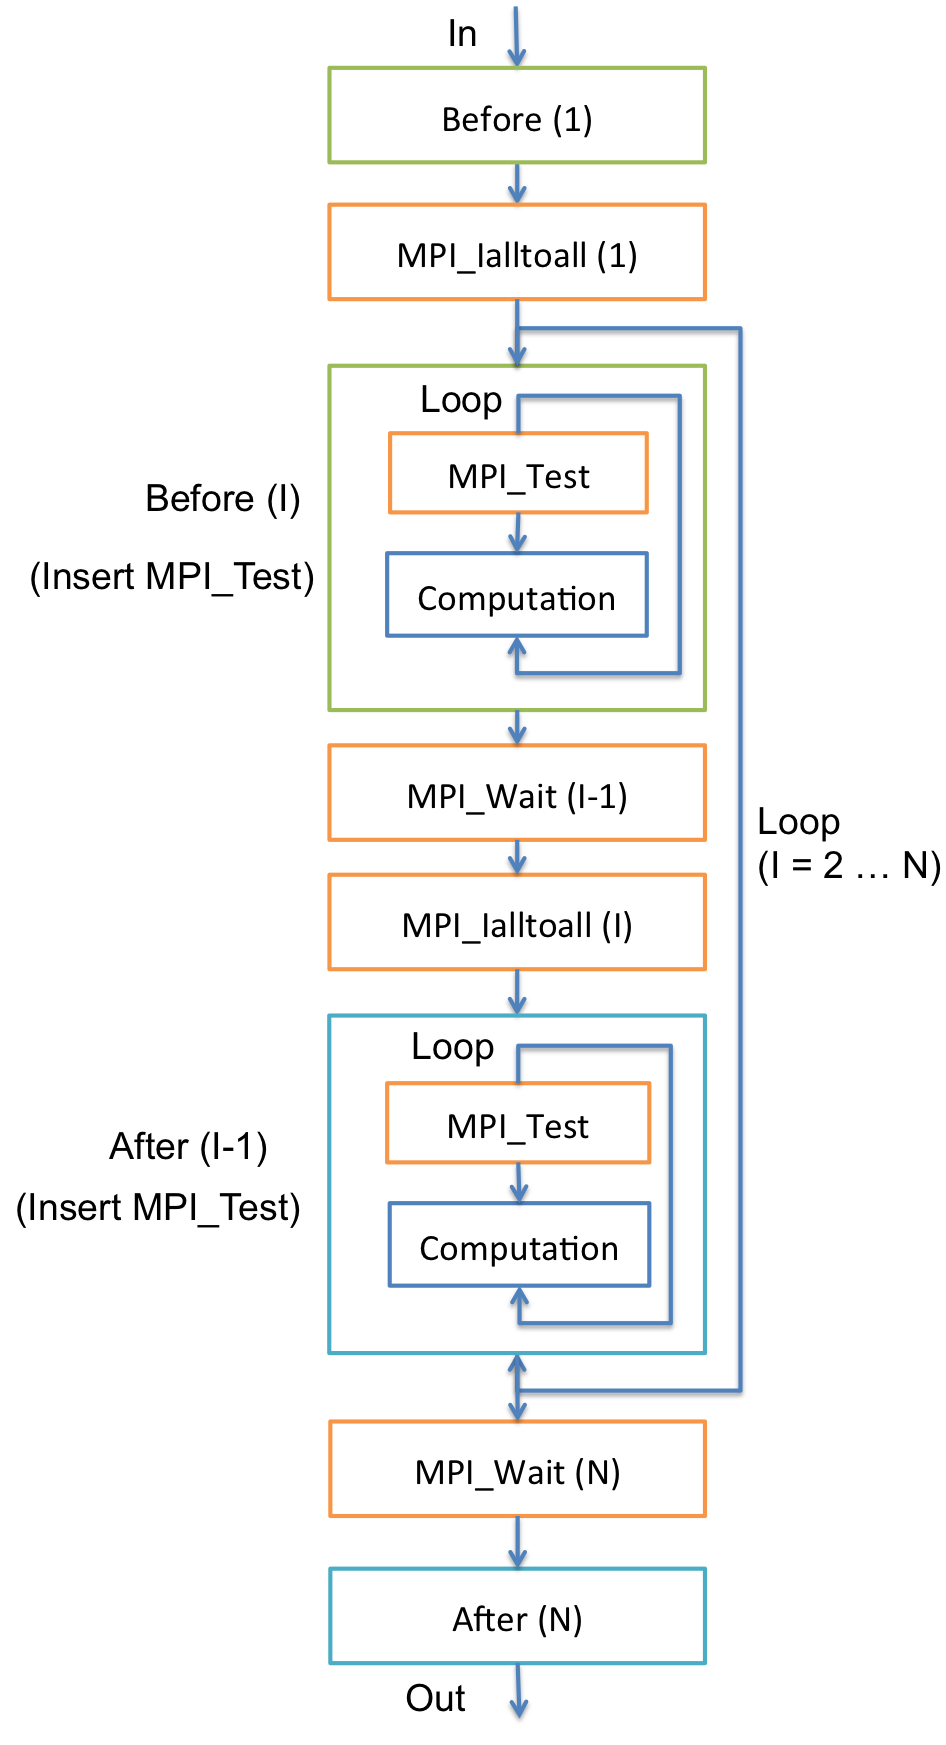
\includegraphics[width=1\textwidth]{fig/ft_cco.png}
    \caption{After optimization}
    \label{fig:ft_cco}
  \end{subfigure}
  \caption{Optimizing NAS FT by
    overlapping computation with communication (Before(i)/After(i) are computations before/after the MPI communication of the $i$th loop iteration)}
\label{fig:ft}
\end{figure}

Figure~\ref{fig:ft_cco} illustrates how the structure
in~\ref{fig:ft_loop} may be modified to better overlap computation
with communication.  In particular, the MPI\_Alltoall operation is
decoupled into two finer-grained operations: a nonblocking
MPI\_Ialltoall and a blocking MPI\_Wait.  Then, the loop is modified
so that Before(i), which multiplies a local matrix with a
time-evolution array and then saves a transpose of the matrix into a
local buffer to be communicated to other processors, and
MPI\_Ialltoall(i), which exchanges the local transposes among different
processes, are essentially moved so that they are evaluated before
$MPI\_Wait(i-1)$, which waits for the completion of MPI communication
of the previous iteration, and $After(i-1)$, which processes the just
received remote data (of the $i-1$th iteration) and then prints the
result into an output file.  By using two distinct buffers to store
the data used in consecutive MPI communications, the output
dependence between After(i-1) and Before(i)/MPI\_Ialltoall(i) can be
eliminated, guaranteeing the correctness of optimization.
%GAIL - it is a bit confusing when and why you use -- and don't use -- italics in the preceding paragraph and later when referring to MPI operations. 

\emph{MPI\_Test} operations then are inserted into the local computation to
ensure the progress of the nonblocking
communication.\footnote{Although MPI communications do not need full
  usage of the CPUs, they need some CPU time, e.g., to manage communication
  progress, which is supplied only when operations such as MPI\_Test
  and MPI\_Wait are invoked.}  By overlapping the MPI communication
with the local computation, the transformed code allows the
application to perform well even on systems with slow network
connections, although nonblocking communications generally take longer
than their blocking counterparts do, and more memory may be needed to
hold the data during communication.

\begin{figure}[h]
\centering
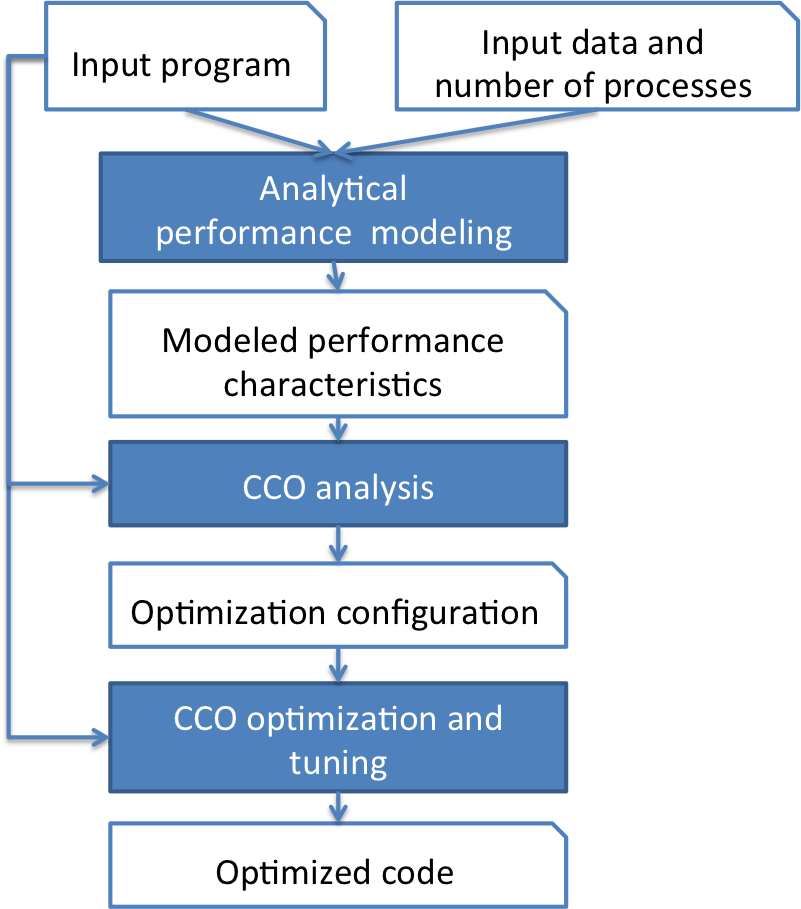
\includegraphics[width=0.35\textwidth]{fig/framework.png} % half page
\caption{Optimization workflow.}
\label{fig:overview}
\end{figure}

Figure~\ref{fig:overview} shows our workflow for systematically
enabling communication-computation overlapping (CCO) in MPI
applications to enhance their performance portability.  The
workflow contains three key components: (1) the \emph{performance
  modeling} component, which analyzes the runtime statistics of an MPI
application to extract a \emph{Bayesian execution
  tree}~\cite{jichi:ipdps14} representation of its execution flow,
including the frequencies of various runtime code paths and their
performance characteristics such as computation intensities, working
set sizes, and communication characteristics of MPI operations; (2)
the \emph{CCO analysis} component, which identifies \emph{hot}
computation and communication regions
and performs profitability and safety
analysis to determine whether to optimize these regions; and (3) the \emph{CCO
  tuning} component, which applies the appropriate program
transformations
%by replacing the blocking MPI operations with
%nonblocking ones, by reordering the computations and communications involved and by inserting
and inserts MPI\_Test operations with a frequency
determined by empirical tuning of the optimized code.
For each optimization to be profitable, any
communication slowdown from the use of the nonblocking operations must
be fully overlapped with the local computation, and the insertion of
MPI\_Test operations should cause only marginal slowdown of the computation.
% so that its effect is insignificant in comparison with the reduction of the original communication time.
Our framework currently
uses empirical tuning to select appropriate
optimization configurations and to skip nonprofitable optimizations.

The idea of overlapping computation and communication in MPI applications has been
well studied~\cite{danalis:sc05,fishgold:ipdps06}, including both using analytical performance
models~\cite{iancu:ppopp07}
and using compiler analysis~\cite{danalis:ics09} to assist the optimization.
Similar to other existing work, we also manually applied the optimizing transformations for each application.
Our work is a step closer to complete automation in that it fully integrates analytical performance modeling and compiler dependence analysis to automatically
determine (with optional developer guidance) the profitability and safety of the overlapping optimization. %, although with some small amount of manual assistance from developers.
The special interprocedural pattern of loop-based
communication-computation overlapping addressed by our work is common in scientific applications but has not been addressed in the literature.
While our example in Figure~\ref{fig:ft} contains only a singe communication inside the loop body, the optimization works similarly
when the body contains a chain of dependent communications, by overlapping them with independent computations of the previous iterations.

%Compared to using profiling to directly measure and identify code blocks to optimize,
% our analytical modeling framework is able to collectively consider all the dynamic paths through each code block,
%to more accurately identify important inter-procedural communication patterns.
Our main technical contributions are the following:

\begin{itemize}

\item Our framework tackles a common case of enhancing the overlapping of computation-communication that has not been previously addressed for MPI applications and
is able to fully automate the profitability and safety analysis of the optimization, by using advanced analytical performance
modeling (which collectively considers all the dynamic paths through each code block) and compiler dependence analysis
(which supports automated semantic inlining of developer-supplied knowledge). Developer guidance is required only to improve the
accuracy of the analysis for large scientific applications, because not all source code
of these applications is available and many low-level implementation details are almost impossible to decipher~\cite{POET:ICPP11}.
 We currently manually apply the necessary program transformations,
  because code need to be carefully moved across procedural boundaries. We believe this process can be automated with some developer
guidance, which is our future work.

\item We applied our approach to optimize 7 NAS Parallel Benchmarks
  (NPB) applications on both a high-speed and a slow network-connected
  cluster environment and achieved 3--88\% speedup on both platforms.

\end{itemize}


The remainder of the paper is organized as follows.
Section~\ref{sec-model} presents our analytical performance modeling
component for automatically identifying communication and computation
hot spots in MPI applications Section~\ref{sec-analysis} discusses how
to automatically determine the safety of the optimization through
compiler analysis.  Section~\ref{sec-opt} summarizes strategies we
used to perform the actual optimizations and the tuning of their
configurations.  Section~\ref{sec-exp} evaluates our framework using 7
NAS application benchmarks~\cite{npb}.  Section~\ref{sec-related}
discusses related work, and Section~\ref{sec-concl} presents our
conclusions.

\section{Analytical Modeling Of MPI Applications}
\label{sec-model}

To effectively reduce the overhead of network communications in MPI
applications, one must understand when and where it becomes beneficial
to enhance the overlap of communications with local computations in
these applications, In particular, through an analytical approach, our
framework aims to model the runtime execution flows of an input
application in terms of their relative amount of time spent in local
computations and network communications.  This information then is
used to automatically identify potential communication bottlenecks as
candidates for optimization in the later steps.

The purpose of our execution flow modeling is to estimate the time
required to complete each MPI communication in relation to adjacent
computations on the local node.  To represent runtime execution paths
and estimate the time required to execute the local computation of
each path, we use the \texttt{Bayesian Execution Tree} (\texttt{BET})
from the Skope analytical performance modeling
framework~\cite{jichi:ipdps14}.  Each BET essentially represents
possible runtime code paths of an application together with their
execution frequency and expected execution time. We use the Skope
framework to automatically generate a BET representation of each
application from the application source code combined with some sample
input data and code-coverage profiling of the application execution.
We then extend the Skope framework to additionally estimate the
overhead of each MPI communication through the following steps.

\begin{enumerate}

\item Use LogGP-based communication model for the MPI runtime to
  estimate the communication time for each individual MPI call.

\item Statistically estimate the expected average communication time
  for each code path by combining the individual communication with
  the execution frequencies.

\end{enumerate}

The balance between the time required for each MPI communication and
the expected execution time of its surrounding local computation is
used to project optimization opportunities. The following first
illustrates the BET representation that we inherit
from~\cite{jichi:ipdps14} and then explains our extensions for
modeling MPI communications.


\subsection {Bayesian Execution Tree}

\begin{figure}[h]
\begin{center}
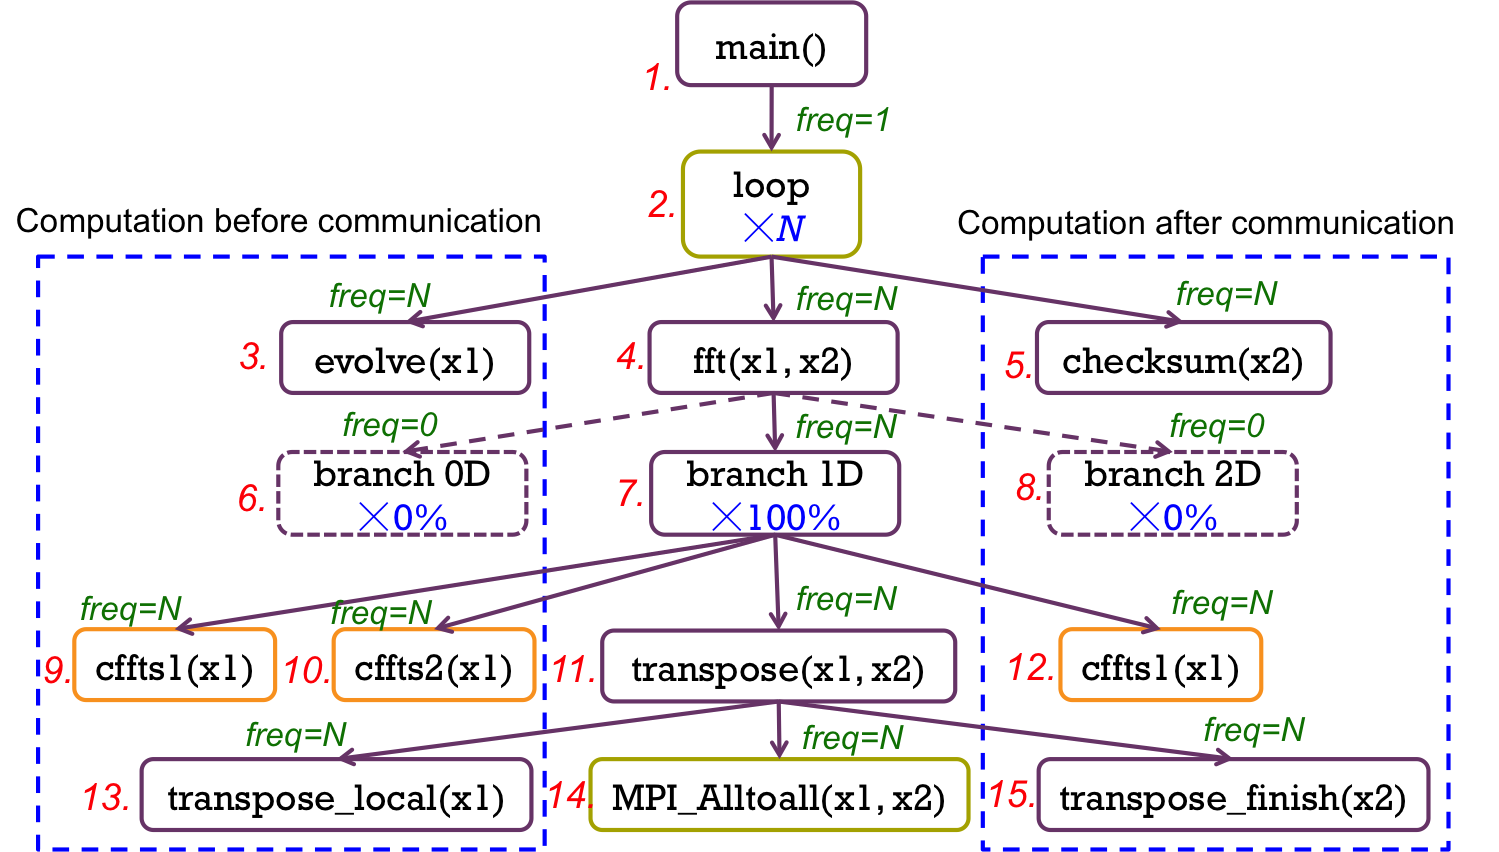
\includegraphics[width=0.48\textwidth]{fig/ft_bet.png}
\caption{Simplified Bayesian Execution Tree for NAS 1D FFT before
  overlapping computation and communications \emph{(for simplicity,
    only important branches, loops, and function calls are shown, and
    not all nodes and frequencies in BET are drawn in this figure)}}
\label{fig:ft_bet}
\end{center}
\end{figure}

Figure~\ref{fig:ft_bet} shows an example \texttt{BET} for one of the
MPI processes of the 1D FFT benchmark in Figure~\ref{fig:ft_loop}.
Each node of the BET represents a code block (a sequence of statements
in the user program) together with its runtime \emph{execution
  frequency}, defined as the expected average number of times that
statements in the node block will be executed at runtime.  A
\texttt{depth-first-traversal} (\texttt{DFS}) of each subtree of the
\texttt{BET} corresponds to a possible runtime execution path of the
statements.  For example, in Figure~\ref{fig:ft_bet}, Node\#2 is a
loop of $N$ iterations, so the frequency of its loop body is $N$.
Node\#7 is a branch inside {\em fft} function. If the application is
to perform 1D FFT, this branch is taken 100\% of time during
execution, so its frequency is $N$, while the frequency of the
alternative branches (Node\#6 and Node\^8) are set to 0.

In order to derive execution frequencies of each code block, the Skope
framework requires a description of the application input data, either
manually provided by the user or automatically collected via an
instrumented run of the application.  The input data description
characterizes the possible values of all the data that the application
may obtain from external sources, for example, command-line arguments,
environment variables, or files.  For array variables, only their
dimensions and the size of dimension are required.  For MPI
applications, the total number of MPI processes
(\texttt{MPI\_Comm\_size}) and the rank of the process to model
(\texttt{MPI\_Rank}) are additionally required.  Based on the input
data description, the Skope framework applies constant propagation to
derive possible values of the expressions that control the directions
of branch and loop controls. A fall-through probability to be 50\% is
assumed if the values cannot be accurately determined.  For this
paper, we used \texttt{gcov} to profile applications with sample input
data,


\subsection{Modeling MPI Communications}

To predict the MPI communication overhead with local
computations, we have extended the Skope framework with the LogGP
model~\cite{loggp} to additionally model the latency (elapsed time) of
each MPI operation using the following four parameters:

\begin{enumerate}

\item $P$: number of processes involved in the communication

\item $n$: size (in bytes)of the message being transferred

\item $alpha$: overhead of starting each message and time interval
  required between transmitting each pair of messages

\item $beta$: expected communication time per byte for large messages,
  determined by the underlying network bandwidth.

\end{enumerate}

Among the four parameters, $alpha$ and $beta$ can be calculated from
characteristics of the underlying network.  In particular, we compute
$beta$ as the reciprocal of the network bandwidth and $alpha$ by using
microbenchmarks to measure the latency of \texttt{MPI\_Send} and
\texttt{MPI\_Recv} operations on the target platform.  The other two
parameters, $P$ and $n$, are either determined through instrumented
runs of the user application or obtained directly from the user as
expected runtime configurations of the application.  In particular,
$P$ equals to \texttt{MPI\_Comm\_size}; and $n$ (i.e., message size)
is obtained from the values used to invoke the MPI operations.

Following the LogGP model, we model MPI point-to-point communications
as:

\begin{equation}
cost_{p2p}(n;alpha,beta) = alpha + n\cdot beta .
\end{equation}

To model the \texttt{MPI\_Alltoal} operation, we use the following two
formulas.

\begin{equation}
  cost_{short} = log P\cdot alpha + \frac{n}{2}\cdot log P\cdot beta
\end{equation}

\begin{equation}
cost_{long} = (P-1)\cdot alpha + n\cdot beta
\end{equation}

The first formula models the communication time of short messages and
the second that of long messages.  We use values of \emph{control
  variables} from the MPI runtime library, for example,
\texttt{MPIR\_CVAR\_ALLTOALL\_SHORT\_MSG\_SIZE} for MPI alltoall, to
determine whether a message should be categorized as {\em short} or
{\em long} and thereby select the proper formulas to use.

After estimating the execution time of each individual MPI operation,
the overall communication time of a code path in BET can be calculated
by adding the communication time of all code blocks along the path,
using the following formula.

\begin{equation}
  cost_{n} = \sum\limits_{i}^{n} cost(i) * freq(i)
\end{equation}

Specifically, the total communication cost of a path of $n$ nodes in
the BET can be computed as the sum of the communication time of each
individual MPI operation multiplied by its execution frequency
$freq(i)$.  Here, $freq(i)$ is calculated by using BET as one of the
properties of the BET node that contains the MPI operation, and
$cost(i)$ is calculated as indicated above using LogGP formulas
instantiated with the expected parameter values of the MPI operations.
For example, the total communication time of \texttt{MPI\_Alltoall} in
Figure~\ref{fig:ft_bet} can be computed by multiplying the average
communication time of \texttt{MPI\_Alltoall} by the number of
iterations of the loop node\#2 ($\times N$) and the fall-through
probability of the 1D FFT branch node\#7 ($\times 100\%$).

\section{Optimization Analysis}
\label {sec-analysis}

The objective of our optimization analysis is to automatically identify which MPI communications to optimize
and  what local computations can be safely overlapped with the communication, through the following three steps.

\begin{enumerate}

\item Analytically identify MPI operations that are potential
  performance bottlenecks based on the modeling of communication cost
  and the execution flow modeling of the entire application described
  in Section~\ref{sec-model}.  In particular, based on the BET
  representation of the user application, this step identifies the top
  $N$ most time-consuming MPI \emph{calls}, which take more than $P\%$
  of the overall communication time, where both $N$ and $P$ are
  user-configurable parameters and were set by default with $N=10$ and
  $P=80$.  The selection is accomplished by simply sorting the
  pre-estimated communication time of all MPI calls in the
  \texttt{BET} and then selecting the top ones.  For example, for the
  NAS FT application shown in Figure~\ref{fig:ft_bet}, a single MPI
  call, the \texttt{MPI\_Alltoall} at the bottom of the BET, is
  selected since it takes more than 95\% of the overall communication
  time.

\item For each identified MPI communication to optimize, select a loop
  of computation that can be potentially overlapped with the
  communication to improve performance, by locating the closest
  enclosing loops of the MPI communication in the \texttt{BET}---for
  example, node\#2 in Figure~\ref{fig:ft_bet} for the NAS FT
  application, to potentially overlap with the communication.  If the
  enclosing loop does not exist, the communication is given up as an
  optimization target.

\item Apply dependence analysis to check the safety of overlapping the
  selected computation and communication.

\end{enumerate}

A key challenge in optimizing large applications is that MPI
communications are often scattered across procedural boundaries and
the computation that can be overlapped with them is often some
distance away and similarly across abstraction boundaries, By using
the Skope framework and through the BET representation of the whole
user application, we are able to inter-procedurally select MPI
communication hot spots as well as their surrounding local
computations as potential optimization targets.
%After using our extended analytical performance modeling of Skope to automatically select 
%the MPI operations to optimize, the loop surrounding each MPI operation can be directly
%located by traversing upwards the BET representation of the application.  
Then, an optimization pragma,  \texttt{\#pragma cco do}, 
illustrated at line~1 of Figure~\ref{fig:code:ft}, is inserted automatically before each selected code region
to instruct the compiler to perform additional analysis to determine the safety of optimization.

We use standard loop dependence analysis within the ROSE C/C++/Fortran compiler~\cite {ROSE} to automatically 
determine the safety of the reordering optimization to each selected code
region and make the compiler inline all function calls within the region when possible; 
that is, when source code of the callee is available. 
For other function calls where inlining is not advisable to the compiler, we insert the following pragmas to provide
additional guidance to the loop dependence analysis. 

\begin{enumerate}

\item \texttt{\#pragma cco ignore}, illustrated at line~3 in
  Figure~\ref{fig:code:ft}, which is manually inserted before each
  function call that can be safely ignored when performing dependence
  analysis. That is, these function calls will not implicate the
  safety of any reordering optimization, when the function call is not
  reachable at runtime but involves I/O statements for debugging
  purposes. Examples of such function calls include the
  $timer\_start()$ and $timer\_stop()$ in Figure~\ref{fig:code:ft}.

\item \texttt{\#pragma cco override}, illustrated at the first line of
  Figure~\ref{fig:annot:a2a} and \ref{fig:annot:ft}, which defines the
  memory side effects of the following function call.  The override
  definitions, if specified, allow dependence analysis to proceed
  across procedural boundaries without actual inlining of the
  procedure implementations. They are also inserted manually but could
  be automatically generated through the integration of advanced
  interprocedural side effect analysis~\cite{kennedy:cpld88}.

\end{enumerate}

The above annotations are currently manually inserted to overcome situations where
traditional function inlining is insufficient to overcome the difficulty
imposed by procedural boundaries, either because the source code of the callee is unavailable 
or the low-level
implementation details of the callee are too complex to be accurately
deciphered by traditional compiler dependence analysis, which is a known issue in compiler analysis~\cite{POET:ICPP11}. 
Figure~\ref{fig:annot:a2a}
shows an example override definition for \texttt{MPI\_Alltoall} in NAS
FT, where we use the $read$ and $write$ pseudo statements to indicate
read and write memory accesses.  Based on the domain knowledge of the
application that send and receive data have atomic types instead of
user-defined types, its memory side effect can be expressed as data
accesses to consequent memories in source and target data.
Figure~\ref{fig:annot:ft} shows another example of the $fft()$
function in NAS FT.  The original function have several branches for
different data layout, while the override definition has only 1D
layout that is the target code path to optimize.

We manually override function inlining according to the following
criteria:

\begin{itemize}

\item The definition of the function is not available or contains too
  many low-level implementation details that are likely to
  overcomplicate the inlined code.  For example, we manually write a
  memory side effect definition for all MPI function calls.

\item The runtime code path of the function call allows the side
  effects of the invocation to be simplified through specialization
  far more than if automatically determined after inlining.  For
  example, in NAS FT, the procedure \texttt{fft} has 6 branches for
  solving different dimensions of the FFT problems (0D, 1D, or 2D),
  while only one branch will be taken for each test.  By manually
  overriding the original definition, we can eliminate the unreachable
  branches.

\item When the same array data are declared with different dimensions
  in the caller and callee, the manual override definition can
  normalize data accesses by converting linearized array accesses to
  easier-to-analyze coordinates.

\end{itemize}


\begin{figure}[h]
{\scriptsize
\begin{verbatim}
1  !$cco do
2  do iter = 1, niter
3    !$cco ignore
4    if (timers_enabled) call timer_start(T_evolve)
5    call volve(u0,u1,twiddle,dims(1,1),dims(2,1),dims(3,1))
6    !$cco ignore
7    if (timers_enabled) call timer_stop(T_evolve)
8    !$cco ignore
9    if (timers_enabled) call timer_start(T_fft)
10   call fft(-1,u1,u2)
11   !$cco ignore
12   if (timers_enabled) call timer_stop(T_fft)
13   !$cco ignore
14   if (timers_enabled) call timer_start(T_checksum)
15   call checksum(iter,u2,dims(1,1),dims(2,1),dims(3,1))
16   !$cco ignore
17   if (timers_enabled) call timer_stop(T_checksum)
18 end do
\end{verbatim}
}
\caption{Source code with directives of the loop in NAS FT to optimize}
\label{fig:code:ft}
\end{figure}

\begin{figure}[h]
{\scriptsize
\begin{verbatim}
$cco override
subroutine fft(dir, x1, x2)
  cffts1(-1,dims(1,3),dims(2,3),dims(3,3),x1,x1,scratch)
  transpose_x_yz(3, 2, x1, x2)
  cffts2(-1,dims(1,2),dims(2,2),dims(3,2),x2,x2,scratch)
  cffts1(-1,dims(1,1),dims(2,1),dims(3,1),x2,x2,scratch)
end subroutine
\end{verbatim}
}
\caption{1D layout code path to override the original $fft()$ definition}
\label{fig:annot:ft}
\end{figure}

\begin{figure}[h]
{\scriptsize
\begin{verbatim}
subroutine transpose_x_yz(l1, l2, xin, xout)
  call transpose2_local(dims(1,l1),
  > dims(2,l1)*dims(3,l1),xin,xout)
  call transpose2_global(xout,xin)
  call transpose2_finish(dims(1,l1),
  > dims(2,l1)*dims(3,l1),xin,xout)
end subroutine
\end{verbatim}
}
\caption{Source code of \texttt{transpose\_x\_yz}}
\label{fig:code:transpose}
\end{figure}

\begin{figure}[h]
{\scriptsize
\begin{verbatim}
subroutine transpose2_global(xin, xout)
  call mpi_alltoall(xin, ntdivnp/np, dc_type, xout,
  > ntdivnp/np, dc_type, commslice1, ierr)
end subroutine
\end{verbatim}
}
\caption{Original source code of \texttt{transpose2\_global}}
\label{fig:code:transpose2}
\end{figure}

\begin{figure}[h]
{\scriptsize
\begin{verbatim}
$cco override
subroutine MPI_Alltoall(sendbuf, sendcount, sendtype,
  > recvbuf, recvcount, recvtype, comm, ierror)
  do i = 1, sendcount
    read sendbuf(i)
  end do
  do i = 1, recvcount
    write recvbuf(i)
  end do
end subroutine
\end{verbatim}
}
\caption{Memory side effect of $MPI\_Alltoall()$ with simple datatype to override its original definition}
\label{fig:annot:a2a}
\end{figure}

% tune.tex
% 9/5/2013 jichi
\section{Program Transformation}
\label{sec-opt}

After selecting the code regions to optimize,
  we currently manually transform the source code to systematically
 enable the overlapping of computation and communication
through the following steps.
%\begin{enumerate}
%\item Function outlining:
%  we split the code region to optimize into \todo { by the communications in it. --- into what subregions? why outlining ?}
%  The interleaved computation and computation are modularized and outlined into functions.
%\item
%Convert blocking communications if existed to non-blocking communication and blocking wait.
%\item Reorder computation and communication by reordering the outlined functions.
%\item
%  If the same data buffer is reused by all loop iterations,
%  we will double the buffers and use different buffers for consequent loop iterations.
%\item
%  We manually insert \texttt{MPI\_Test} into the outlined computation function, and adjust their frequencies to get the best performance.
%  If there is only one communication in the code region, the insertion of \texttt{MPI\_Test} is indispensable to have speed-up.
%\end{enumerate}

\subsection{Function outlining}
Given a loop to optimize, we
first outline the computation and communication inside the loop into separate functions,
in order to make it easier to replicate and reorder them later into different loop iterations. In particular, we divide the statements at each iteration I of the target loop into the MPI communications at iteration I (Comm(I)),
the computation  (Before(I)) that should run before Comm(I), and the computation (After(I)) to evaluate after Comm(I)
Each group of statements is then outlined into a separate procedure,  with the loop index variables as its function parameters.\footnote{These components can alternatively be simply tagged as Comm(I), Before(I), and After(I) if the optimization were to be fully automated; outlining makes it easy to modify the code manually.}
Take NAS FT in Figure~\ref{fig:ft_loop} as an example.  The loop to optimize is divided into
  $Comm(I)$, the MPI communication at iteration I;
  $Before(I)$, the computation before communication at iteration I;
  and $After(I)$, the computation after communication at iteration I.

\subsection{Converting MPI communications}
Each blocking MPI operation, for example, {\em alltoall} collectives and point-to-point send-receives,
is converted to an equivalent nonblocking communication combined with a blocking wait.
For example,  in Figure~\ref{fig:ft_loop}, the outlined communication function $Comm(I)$,  which invokes $MPI\_Alltoall$ internally, is replaced by $Icomm(I)$ and $Wait(I)$, which are the corresponding nonblocking communication ($MPI\_Ialltoall$) and wait operations converted from $Comm(I)$, respectively.

\subsection{Reordering computation and communication}

After the previous steps, the body of the loop to optimize now contains a sequence of specially
named operations such as
 $Before(I)$, $After(I)$, $Icomm(I)$, and $Wait(I)$,
  where $I$ is the loop index variable looping from $1$ to $N$.
%
% 1:
%   Loop I = 1 .. N
%   - Before(I)
%     Comm(I)
%     After(I)
%
% 2:
%   Loop I = 1 .. N
%   - Before(I)
%     Icomm(I)
%     Wait(I)
%     After(I)
%
% 3:
%   Before(1)
%   Icomm(1)
%   Loop I = 2 .. N
%   - Wait(I - 1)
%     After(I - 1)
%     Before(I)
%     Icomm(I)
%   Wait(N)
%   After(N)
%
% 4:
%   Before(1)
%   Icomm(1)
%   Loop I = 2 .. N
%   - Before(I)
%     Wait(I - 1)
%     Icomm(I)
%     After(I - 1)
%   Wait(N)
%   After(N)
%
We then %\emph{shift}
  \emph{interleave} the communication and computation operations of consecutive loop iterations,
  as illustrated in Figure~\ref{fig:cco:reorder},  in two steps:
\begin{enumerate}
\item Move $Before(1)$ and $Icomm(1)$ to the outside before the first iteration of the loop starts,
  and move $Wait(N)$ and $After(N)$ outside after the last loop iteration
  as shown in Figure~\ref{fig:cco:reorder:c}.
\item Move $Before(I)$ and $Icomm(I)$ above $Wait(I-1)$ and $After(I-1)$
  as shown in Figure~\ref{fig:cco:reorder:d}.
\end{enumerate}
After the reordering, the nonblocking communication in the current iteration I (between $Icomm(I)$ and $Wait(I)$)
   can be processed in parallel with the computation in the previous ($After(I-1)$) and next ($Before(I+1)$) iterations.

\subsection{Replicating the communication buffer}
Each MPI operation needs a dedicated buffer to hold the data being communicated.
Applications typically first allocate the necessary communication buffers at the initialization stage and then reuse
the same buffers in the same MPI operations across different loop iterations.
After applying our optimization, as illustrated in Figure~\ref{fig:cco:shift},
  the communication ($Icomm(i)$ and $Wait(i)$) at each $i$th iteration, where $i \geq 2$,  is overlapped with computation $Before(i+1)$ and $After(i-1)$.
  Assuming that two distinct buffers, {\em InBuf} and {\em OutBuf}, are used for sending and receiving each message, respectively, 
 each buffer needs to be replicated into a pair of equal size to ensure that distinct buffers are used across the overlapping iterations, 
as illustrated in Figure~\ref{fig:cco:dup}.
%In the figure, the $InBuf$ and $OutBuf$ represent the memory of the send/receive data of the communication $Icomm$ shared by all loop iterations.
In particular, we replicate each buffer
  by allocating additional memory outside the loop %that has the same size of the original data buffers
  and then alternately use a distinct buffer in every pair of consecutive loop iterations.
% GWP - do you mean alternately?

%n particular, for each buffer used by $Comm(I)$ that used by the overlapping computation, a new buffer of the same size is created;
%  and then replace the buffers accessed at the odd iteration by the communication
%                   and those accessed at the even iteration by the computation
%  with the replicated buffers.

\subsection{Inserting MPI\_Tests}
% 1. Multi-threaded communication:
% Put computation on one thread, and put communication on the other thread.
% We can explicitly create threads for computation and communication.
% Additionally, the MPI implementation also support implicitly and automatically put the whole background communication onto another thread.
% For example, when we compile MPICH3, there is actually a flag for whether we want to enable this or not. And this threading flag is disabled by default.
%
% When threading exist, there is no need to do MPI_Test to overlap the computation and communication.
%
% 2. Single-threaded communication:
% Put both computation and communication on the thread, which is the typical configuration of MPI.
% In this scenario, to overlap computation with long communication, we need frequently call MPI_Test in the middle of computation to continues poll the MPI communication engine.
%
% However, if the communication itself takes very short time, then calling MP_Test might have no impact and could slowdown the overall performance.

When using nonblocking MPI operations, some CPU time needs to be allocated, by embedding $MPI\_Test$ calls in the local computation,
to ensure continuous progress of the communications.
If the local computation is not inside a loop, we insert one or more $MPI\_Test$ calls evenly distributed into the computation.
%And if insertion of $MPI\_Test$ cause slowdown, it will be removed instead.
On the other hand, if the local computation is inside a loop,
  we insert $MPI\_Test$ into the beginning of the loop body and use a conditional variable to adjust its frequency.
The inserted code is illustrated in Figure~\ref{fig:cco:test}.
In both cases, the frequency of $MPI\_Test$ is empirically adjusted as the application is ported to each architecture.


% https://en.wikibooks.org/wiki/LaTeX/Floats,_Figures_and_Captions
\begin{figure}
{\scriptsize
  \centering
  \begin{subfigure}[b]{.25\textwidth}
\begin{verbatim}
DO I = 1 .. N
  Before(I)
  Comm(I)
  After(I)
END DO
\end{verbatim}
    \caption{Input loop}
    \label{fig:cco:reorder:a}
    \vspace{.1in}
  \end{subfigure}%
  \begin{subfigure}[b]{.25\textwidth}
\begin{verbatim}
DO I = 1 .. N
  Before(I)
  Icomm(I)
  Wait(I)
  After(I)
END DO
\end{verbatim}
    \caption{Decouple blocking comm}%unication
    \label{fig:cco:reorder:b}
    \vspace{.1in}
  \end{subfigure}
  \begin{subfigure}[b]{.25\textwidth}
\begin{verbatim}
Before(1)
Icomm(1)
DO I = 2 .. N
  Wait(I - 1)
  After(I - 1)
  Before(I)
  Icomm(I)
END DO
Wait(N)
After(N)
\end{verbatim}
    \caption{Move first and last iterations}
    %\caption{Loop with iterative computation and communication}
    \label{fig:cco:reorder:c}
  \end{subfigure}%
  %add desired spacing between images, e. g. ~, \quad, \qquad, \hfill etc.
  %(or a blank line to force the subfigure onto a new line)
  \begin{subfigure}[b]{.25\textwidth}
\begin{verbatim}
Before(1)
Icomm(1)
DO I = 2 .. N
  Before(I)
  Wait(I - 1)
  Icomm(I)
  After(I - 1)
END DO
Wait(N)
After(N)
\end{verbatim}
    \caption{Interleave consequent iterations}
    %\caption{Decouple and overlap the communication of the i-th iteration with the computation of the (i-1)-th and (i+1)-th iterations}
    \label{fig:cco:reorder:d}
  \end{subfigure}
\caption{Steps to reorder outlined communication and computation functions}
\label{fig:cco:reorder}
}%\scriptsize
\end{figure}

\begin{figure}
{\scriptsize
  \centering
  \begin{subfigure}[b]{.20\textwidth}
\begin{verbatim}
Before(1, InBuf)
Icomm(1, InBuf)
DO I = 2 .. N
  Before(I, InBuf)
  Wait(I - 1)
  Icomm(I, InBuf
         , OutBuf)
  After(I - 1, OutBuf)
END DO
Wait(N, OutBuf)
After(N, OutBuf)
\end{verbatim}
    \caption{Original communication that uses the same input and output $Buf$}
    \label{fig:cco:dup:a}
  \end{subfigure}%
  \hspace{.01in}
  \begin{subfigure}[b]{.28\textwidth}
\begin{verbatim}
Before(1, InBuf)
Icomm(1, InBuf)
DO I = 2 .. N
  Before(I, I % 2 ==  1 ? InBuf : InBuf2)
  Wait(I - 1)
  Icomm(I, I % 2 ==  0 ? InBuf : InBuf2
         , I % 2 ==  0 ? OutBuf : OutBuf2)
  After(I - 1, , I % 2 ==  1 ? InBuf : InBuf2)
END DO
Wait(N, N % 2 == 1 ? OutBuf : OutBuf2)
After(N, N % 2 == 1 ? OutBuf : OutBuf2)
\end{verbatim}
    \caption{Replicate $Buff$ with $Buff2$ of the same size}
    \label{fig:cco:dup:b}
  \end{subfigure}
\caption{Replicate communication buffers for nonblocking communication}
\label{fig:cco:dup}
}%\scriptsize
\end{figure}

\begin{figure}[h]
{\scriptsize
\begin{verbatim}
DO I = 1 ... L
  If I % Freq == 0
    MPI_Test
  Original_computation_statements
END DO
\end{verbatim}
}%\scriptsize
\caption{Insert MPI\_Test into the hot computation loop at specific frequency $Freq$}
\label{fig:cco:test}
\end{figure}

\begin{figure}[h]
\centering
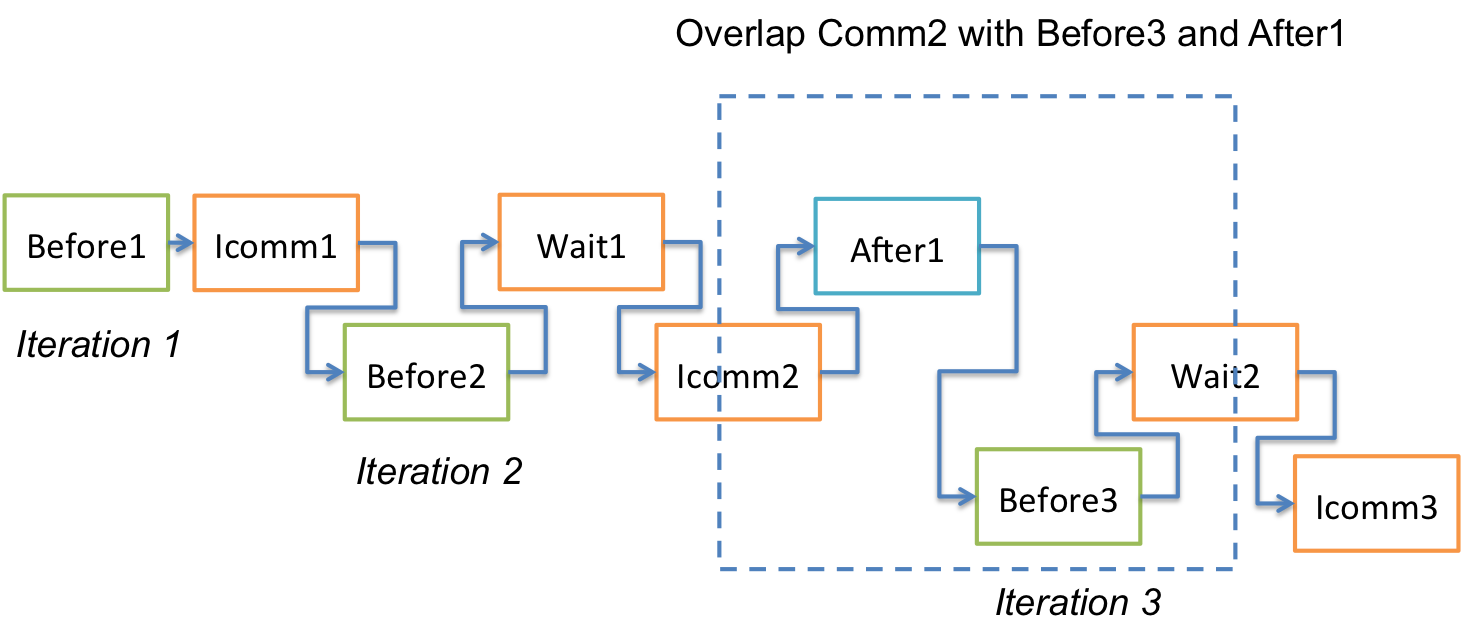
\includegraphics[width=0.49\textwidth]{fig/ft_shift.png} % half page
\caption{Overlapped computation and communication operations}
\label{fig:cco:shift}
\end{figure}

%We insert MPI\_Test into four out of all eight NAS benchmarks.

% EOF

%\begin{figure}
%\centering
%{\scriptsize
%  \begin{subfigure}[b]{0.2\textwidth}
%\begin{verbatim}
%MPI_Ialltoall
%Loop I = 1 ... L
%  If I % Freq == 0
%    MPI_Test
%  Computation
%MPI_Wait
%\end{verbatim}
%  \caption{Single computation loop}
%  \label{fig:cco_test:single}
%  \end{subfigure}%
%  \begin{subfigure}[b]{0.3\textwidth}
%\begin{verbatim}
%MPI_Ialltoall
%Loop I = 1 ... L1
%  If I % Freq1 == 0
%    MPI_Test
%  Computation1
%Loop I = 1 ... L2
%  If I % Freq2 == 0
%    MPI_Test
%  Computation2
%...
%Loop I = 1 ... LN
%  If I % FreqN == 0
%    MPI_Test
%  ComputationN
%MPI_Wait
%\end{verbatim}
%  \caption{Multiple computation loops}
%  \label{fig:cco_test:multiple}
%  \end{subfigure}%
%\caption{Single or multiple computation loops with MPI\_Test inserted}
%\label{fig:cco_test}
%}%\scriptsize
%\end{figure}
%If MPI\_Test is in loops,
%  a condition will be inserted before the MPI\_Test as shown in Figure~\ref{fig:cco_test}
%  to control how many MPI\_Test to execute in the loops, or the \emph{frequency} of MPI\_Test.
%When there are multiple computation loops to insert MPI\_Test,
%  multiple frequencies are needed to be inserted.
%Our experiment results show
%  when MPI\_Test is evenly distributed in the computation time,
%  it can achieve the best performance.
%To make the computation statements in between each pair of MPI\_Test to have roughly equal computation time,
%  the MPI\_Test frequencies are determined by the estimated computation time for loops using analytical modeling
%  so that given two loops L1 and L2:
%\begin{equation}
%  time(Computation_1) * Freq_1 = time(Computation_2) * Freq_2
%\end{equation}
%Given the above relation, the frequencies of multiple MPI\_Test can be control by a single frequency,
%  which is then tuned using binary search on the target runtime environment,
%  i.e. the frequency is constantly increased/decreased when the total execution time is reduced.

%All the point-to-point (send and receive) and collective communication (broadcast, reduce, allreduce, alltoall)
%  being considered in the MPI standards have both blocking and non-blocking functions.
%A blocking function (such as \texttt{MPI\_Alltoall}) can be replaced by a non-blocking function (such as \texttt{MPI\_Ialltoal})
%  and a wait (\texttt{MPI\_Wait}).
%Because \texttt{MPI\_Request} used to connect the non-blocking function and wait
%5  will also be needed by \texttt{MPI\_Test},
%  is is made as a global variable to make it easier to pass to MPI\_Test.
%After decoupling blocking communication, the $Comm$ function will be replaced by $Icomm$ and $Wait$ as shown in Figure~\ref{fig:ft_cco}.

%The variables in the optimization configuration that might carry loop-carried dependence
%  are privatized for each loop iteration.
%If the variables are used as output,
%  the value of the privatized variables are copied to the output variables at the end of each loop iteration.

%To insert the computation in between the decoupled communication,
%  the outlined/specialized computation and communication functions will be reordered
%     as shown in Figure~\ref{fig:ft_cco}.

%Taking the estimated overlap code region by analytical modeling,
%the goal of the CCO analysis stage
%  is to find the computation statements that can be potentially overlapped with the communication.
%There are two ways to overlap the communication and computation.
%The first is to move the computation into the middle of the communication region,
%and (2) interweave the communication and communication loops if both of them are in loops.
%The first one requires the computation that can be safely reordered with the communication;
%and the second one need the computation and communication loops to be fusible.
%Correspondingly, the target computation statements can be divided into two categorized
%  based on their dependence relation to the communication to overlap:
%\begin{enumerate}
%\item Independent computation statements, which are independent from the communication to overlap.
%These statements are able to be reordered freely with the communication in the later program transformation stages.
%\item Decomposable computation loops, which can be safely merged with the communication loops.
%Although there dependence edges between the computation and the communication,
%but after loop fusion, there are no loop carried dependence between communication and communication in the result code.
%As the result, the communication loops and communication can be possibly interwoven.
%\end{enumerate}
%In order to be able to overlap the computation with the communication,
%the computation statements are needed to be \emph{surrounding} with the communication
%that for reach computation statement,
%there is a runtime code path between the computation and a communication
%where all statements on the code path are either independent or decomposable statements.
%%The independent and decomposable workflow is a list of statements
%%  that are either independent from all communication,
%%  or can be decomposable in the same way as the group of communication.
%
%The following subsections will first
%describe the rules to determine independent and decomposable statements,
%then discuss the algorithm to find them in the specified overlap code region.


%The data dependence between a communication and a computation statement
%  is a situation in which one statement refers to the data of the other preceding statement.
%This relation can be determined by analyzing the memory side effects of the statements.

%\subsection{Computing independent and decomposable workflow}

%\subsection{Independent computation}
%An independent computation statement in the overlap code region
%is independent from all communication in the region,
%which means that
%for each communication in the code region,
%there are neither direct nor transitive dependence between the communication and the independent computation.
%The relation could be formally stated as that
%given a independent communication statement $A$ and overlap region $R$,
% independent if for each communication statement $B$ in $R$,
%  there are neither direct nor transitive dependence edge between $A$ and $B$.

%Given this definition, the independent statement can be computed using data dependence analysis.
% Independent condition
%Given a computation and a communication,
%  if there is data dependence between them,
%  they must be both decomposable to loops in order to overlap them.
%
%Assume the computation statement is decomposable to loop $L_1$,
%  and loop $L_2$ is one of the loops that the communication can be decomposed to.
%If loop $L_1$ and $L_2$ can be fused,
%  then the computation and communication are compatible and able to be overlapped after the decomposition.
%
%The communication group could be either a single collective communication,
%  or a list of decoupled send/receive and blocking/non-blocking communication.
%The communication group can be decomposed if the communication statements in the group
%  can be transformed into a loop.

% Communication decomposition
%The CCO analysis stage will select the optimization configurations to apply
%  and the configurations into source code as \emph{CCO annotations}.
%The analysis takes the source code,
%   application's code skeleton,
%   and the hardware performance model as input.
%The optimization configurations include
%  the decomposition patterns for the communication
%  and the functions needed to inline.
%The overall workflow is illustrated in the Figure~\ref{alg:analysis}.


%\subsection{Computing overlappable computation}
%
%The overlappable computation is either
%statements that are independent from the communication,
%or the loops that are fusible with he communication loops.
%Additionally, the computation must be \texttt{reachable} by the communication
%that there is a runtime code path between the computation and the communication
%where all statements on the code path are either independent or decomposable statements.
%Given these requirements,
%  the overlappable computation can be computed using the data-flow analysis and control flow analysis
%  by the following two stepts:
%\begin{itemize}
%\item First, find the first and the last communication in the code region.
%\item Then, traverse the control flow for each statement before the first or after the last communication.
%  If the statement is either independent from or decomposable to the communication,
%  then identify it as overlappable; otherwise stop the traversal.
%\end{itemize}

%Additionally, the compatible computation loop must be \textbf{reachable} by the communication in order to overlap them.
%Given a computation loop $L$ that is compatible with the decomposable communication group $G$.
%In order to overlap them, there must be a list of statements $F$ in the control flow between them
%  where all the statements are in the same code block, or can be moved into the same code block.
%And the statement list $F$ must satisfy one of the following conditions:
%\begin{enumerate}
%\item All statements in $F$ are independent from $G$.
%\item All statements in $F$ are loops that are compatible with $G$.
%\item $F$ can be partitioned into two sub lists.
%The list connecting $G$ are independent from $G$.
%The other list connecting $L$ are loops that are compatible with $G$.
%\end{enumerate}
%The statement list $F$ can be computed in the way similar to that to find the overlap scope stage.
%We can traverse in the overlap code region from $G$ to compute $F$.
%First, if the parent blocks of $G$ are simple blocks that are not loops, branches, and functions,
%  the block boundaries can be eliminated by merging the parent blocks.
%Then, the parent block of $G$ can be divided into two statement lists:
%  one before $G$ and one after $G$.
%Because there are no function calls in the code region after annotation-based inlining,
%  the block of procedure boundary are not needed to be considered.
%% Group of independent statements
%% reachability
%If the group is a list of decoupled communication statements,
%  it can be decomposed if the communication statements are in the same loop.
%If the group is a collective communication,
%  it can be decomposed if the collective communication can be divided into a loop of point-to-point communication.
%There could be different possible ways to decompose a collective communication
%  depending on the portion of data and message size assigned to each point-to-point communication.
%
%The independent and decomposable workflow is a list of statements
%  that are either independent from all communication,
%  or can be decomposable in the same way as the group of communication.
%
%The data dependence between a communication and a computation statement
%  is a situation in which one statement refers to the data of the other preceding statement.
%This relation can be determined by analyzing the memory side effects of the statements.

%A computation statement can be decomposed if it is a loop, or can be transformed into a loop.
%Depending on where the loop is, it can be categorized into the following scenario:
%\begin{itemize}
%\item The statement is a loop.
%\item The loop is in the statement generated by function alls.
%\end{itemize}
%To describe the data access of the decomposed loop,
%  the decomposition can be described as a tuple of
%  $(I, D, P)$ where
%  $I$ is the loop iteration,
%  $D$ is the data accesses per iteration with loop-carried dependence,
%  and $P$ is the  data accesses per iteration without loop-carried dependence.
%Similar to the computation decomposition,
%  the communication decomposition can also be described as the tuple of $(I,D,P)$ for the decomposed loop.
%The difference is that if the communication group is a collective communication,
%  then $D = \emptyset$,
%  and there could be multiple possible $(I,P)$ combinations that could become a decomposition space.
%So, the ways to decompose collective communication could be described as $\{(I,P)\}$, a set of all possible $(I,P)$.
%Given a computation statement $X$ decomposable to $(I,D,P)$,
%and a communication group $Y$ that can be possibly decomposed to any of $\{(I_i,D_i,P_i)\}$,
%then $X$ and $Y$ are compatible if $(I,D,P)$ and any $(I_i,D_i,P_i)$ satisfy any of the following requirements
%(let $W(D)$ represents the write data accesses in $D$):
%\begin{itemize}
%\item $I = I_i$ and $W(D) \cap (D_i \cup P_i) = \emptyset$ and $W(D_i) \cap (D \cup P) = \emptyset$
%\item $I \% I_i = 0$ and $W(D_{tile}) \cap (D_i \cup P_i) = \emptyset$ and $W(D_i) \cap (D_{tile} \cup P_{tile}) = \emptyset$,
%  where $D_{tile}$ and $P_{tile}$ are $D$ and $P$ tiled by $I/I_i$.
%\end{itemize}
%The formal definitions for the reachability is as follows.
%
%Let $C$ be the set of communication statements to overlap.
%Let $S$ be the decomposable communication code represented by a \texttt{BET} statement which is defined as follows:
%\begin{itemize}
%\item If $C$ contains only one collective communication $X$, let $S$ be $X$.
%\item Else if all communication in $C$ are in the same loop $X$, let $S$ be $X$.
%\item Otherwise, the communication cannot be decomposed for overlapping, and $S$ does not exist.
%\end{itemize}
%Let $R$ be the set of statements in the overlap code region.
%Let $I$ be the set of an independent statements to compute.
%A recursive definition of $I$ is as follows:
%\begin{itemize}
%\item Let $X$ be any communication statement in $C$.
%  For each sibling node $Y$ of $X$ in $R$, if $Y$ is independent of $X$, add $Y$ to $I$.
%\item Let $X$ be any communication statement in $C$, and $Z$ be any node in $I$.
%  For each sibling node $Y$ of $Z$ in $R$, if $Y$ is independent of $X$, add $Y$ to $I$.
%\item If $S$ exists, for each sibling node $Y$ of $S$ in $R$, if $Y$ is independent of $S$, add $Y$ to $I$.
%\end{itemize}
%Let $D$ be the set of decomposable statement to compute.
%If $S$ does not exist, which means the communication can not be decomposed, then $D$ is empty.
%Otherwise if $S$ exists, a recursive definition of $D$ is as follows:
%\begin{itemize}
%\item For each sibling node $Y$ of $S$ in $R$, if $Y$ can be decomposed in the same way of $S$, add $Y$ to $D$.
%\item Let $X$ be any decomposable statement in $D$.
%  For each sibling node $Y$ of $X$ in $R$, if $Y$ can be decomposed in the same way of $S$, add $Y$ to $D$.
%\item Let $X$ be any independent statement in $I$ that is outside of $S$.
%  For each sibling node $Y$ of $X$ in $R$, if $Y$ can be decomposed in the same way of $S$, add $Y$ to $D$.
%\end{itemize}
%
%Given two statements $S_2$ and $S_2$.
%Let notation $R(S)$ be the set of data that statement $S$ could read.
%Let notation $W(S)$ be the set of data that statement $S$ could write.
%The relations of the independence and decomposition between two single statements are defined as follows:
%\begin{itemize}
%\item Independence:
%  $S_1$ and $S_2$ are independent if:
%  $R(S_1) \cap W(S_2) = \emptyset \wedge W(S_1) \cap R(S_2) = \emptyset \wedge W(S_1) \cap W(S_2) = \emptyset$.
%\item Decomposition:
%  Let $D = (R(S_1) \cap W(S_2)) \cup (W(S_1) \cap R(S_2)) \cup (W(S_1) \cap W(S_2))$ be the shared data access between the two statements.
%  $S_1$ and $S_2$ can be decomposed in the same way if they satisfy the following requiremens:
%    \begin{enumerate}
%    \item $D \ne \emptyset$
%    \item $S_1$ can be decomposed into a loop. Let $D_1(i)$ be the data in $D$ accessed by the loop body at iteration $i$.
%    \item $S_2$ can be decomposed into a loop. Let $D_2(i)$ be the data in $D$ accessed by the loop body at iteration $i$.
%    \item For any two loop iterations $i$ and $j$: $D_1(i) \cap D_1(j) = \emptyset$.
%    \item For any two loop iterations $i$ and $j$: $D_2(i) \cap D_2(j) = \emptyset$.
%    \item For any loop iteration $i$: $D_1(i) = D_2(i)$.
%    \end{enumerate}
%\end{itemize}


%The problem to decompose the computation and communication in the way that they can be overlapped
%  could be divided into three sub-problems.
%\begin{enumerate}
%\item If it is possible and how to decompose a computation statement
%\item If it is possible and how to decompose the communication group
%\item If it is possible and how to overlap a decomposed computation and communication
%\end{enumerate}
%
%For a computation statement, if it is a loop, it has been decomposed.
%For a collective communication statement, it can be decomposed into a loop of point-to-point communication.
%For a group of point-to-point communication, if their enclosing block is a loop, they has been decomposed.
%
%Given a decomposable computation statement and a decomposable communication group,
%  they can be overlapped if their decomposed loops can be fused.
%Let $L_1$ and $L_2$ be the two decompose loops.
%Let $D$ be the set of data that $L_1$ depends on $L_2$.
%Then, $L_1$ and $L_2$ can be fused if they satisfy the following requirements.
%\begin{enumerate}
%\item There is no loop-carried dependence of $D$ in both $L_1$ and $L_2$.
%\item The data access of $D$ in $L_1$ is equals to or a subset of that in $L_2$'s body.
%\end{enumerate}
%
%
%The output of the independent workflow could be represented by a set of statements
%  where all statements in the set are independent from all communication.
%The output of the decomposable workflow could be represented by a set of statements
%  where all statements in the set can be decomposed together with the communication group in the same way.
%Formal definitions of the concepts are as follows.
%
%The purpose is to compute the computation that are either independent from the communication, or can be decomposed in the same way as the communication.
%There must be on an execution flow $F$ between the communication $A$ and the computation $B$,
%% all statements \textbf{can be transformed into the same block}.
%which satisfies one of the following conditions:
%\begin{itemize}
%\item All statements in $F$ (including $B$) are independent from $A$
%\item There is a statement $S$ in $F$ that can cut $F$ into two segments that all statements between $A$ and $S$ (including $S$) are independent from $A$, and all statements between $S$ and $B$ (including $B$) can be decomposed in the same way as $A$.
%  %or grouped together at the end of the independent execution flow.
%\end{itemize}
%
%\begin{itemize}
%\item Input from within the framework
%  \begin{itemize}
%  \item The overlap region
%  \item Dependence graph for the overlap region
%  \item The communication group to overlap
%  \end{itemize}
%\item Output: Reachable independent and decomposable computation and communication which can be overlapped later
%\end{itemize}
%An example from NAS FT about the reachable path for decomposable statements are as follows.
%The path connecting the decomposable Alltoall communication with the computation is as follows:
%\begin{equation}
%cffts1 \Rightarrow transpose\_xy\_z \Rightarrow transpose2\_local \Rightarrow transpose2\_global
%\end{equation}
%
%{\scriptsize
%\begin{verbatim}
%subroutine FT
%  if (layout_type .eq. layout_1d) then // This is the overlap region
%    call cffts1(1, dims(1,1), dims(2,1), dims(3,1), // Level = 0, inline
%>               x1, x1, scratch)
%    call transpose_xy_z(2, 3, x1, x2)    // Level = 0, inline
%    call cffts2(1, dims(1,3), dims(2,3), dims(3,3),
%>               x2, x2, scratch)
%
%subroutine cffts1(is, d1, d2, d3, x, xout, y) // Level = 0, inline
%  // Decomposable computation hot spot
%  do k = 1, d3
%     do jj = 0, d2 - fftblock, fftblock
%        do j = 1, fftblock
%           do i = 1, d1
%              y(j,i,1) = x(i,j+jj,k)
%           enddo
%        enddo
%        call cfftz (is, logd1, d1, y, y(1,1,2))
%        do j = 1, fftblock
%           do i = 1, d1
%              xout(i,j+jj,k) = y(j,i,1)
%           enddo
%        enddo
%     enddo
%  enddo
%  return
%  end
%
%subroutine transpose_xy_z(l1, l2, xin, xout) // Level = 0, inline
%  call transpose2_local(dims(1l1)*dims(2,l1),dims(3,l1), // Decomposable
%> xin,xout)
%  call transpose2_global(xout,xin) // Decomposable communication
%  call transpose2_finish(dims(1,l1)*dims(2,l1),dims(3,l1)
%> xin,xout)
%  return
%  end
%
%
%\end{verbatim}
%}%\scriptsize
%
%% Safety analysis
%\subsection{Safety analysis}
%
%The safety analysis is used to determine if the computation and communication workflows are safe to overlap,
%  and to find possible decomposition patterns for the communication.
%The analysis is based on data flow analysis.
%
%\subsubsection{Symbolic representation of data access patterns}~
%We summarize the data access patterns for each node in \texttt{BET}
%  for safety analysis later.
%The data access patterns contains the array being read and written
%  and the symbolic representation of the data being accesses.
%If the node is a nested loop,
%  the access pattern contains the data being accessed in each iteration in the inner loops;
%otherwise
%  the access pattern is the ranges of data being accessed.
%
%For example, the data access pattern for the two computation loop nests in the Figure~\ref{fig:ft} are:
%\begin{itemize}
%\item $ld\ xin[j][k][i]$ and $st\ xout[j][k][i]$ where $j=1:d2,k=1:d3,i=d1$.
%\item $ld\ xin[j][k][i]$ and $st\ xout[j][k][i]$ where $k=1:d3$.
%\end{itemize}
%
%\subsubsection{Summarize data access patterns for BET node}~
%
%The array accesses in BET are expressed by \texttt{ld} and \texttt{st} to array elements.
%The data access patterns for BET node are summarized by traversing the array accesses in the child nodes.
%If the node is a nested loop, the accesses are symbolized to the loop iteration variables.
%Otherwise, the access patterns are expressed as sets of elements that can be read or modified in node.
%
%%\subsubsection{Loop interchange}
%
%\subsubsection{Mapping array indices between procedures}~
%
%In scientific applications, %especially in \texttt{Fortran} language,
%  the same array could have different address spaces.
%In BET, each node has the information of the array dimensions in the data access patterns.
%The dataflow from one procedure to another could be calculated by mapping
%  different address spaces of the two procedures.
%

% exp.tex
% 9/5/2013 jichi

\section{Experiment Results}
\label{sec-exp}
To evaluate the accuracy of our hot-spot communication predictions
  and the performance implications of our manually applied optimizations to better overlap computation with communication,
we applied our approach to model and optimize 7 MPI applications from the NAS NPB~\cite{npb}
  on two clusters shown in Figure~\ref{tab:hw}.
The first Intel platform is a large high-performance computing cluster with very fast internode communication through InfiniBand.
  The second platform is in a small data center where the internode communication is through relatively slow Ethernet.
Both clusters use MPICH 3.1.1~\cite{mpich2} as the underlying MPI library.
Because our current analytical performance model cannot estimate intranode MPI communication time,
  we have allocated a single MPI process per node on both clusters.
  % so that MPI communication is inter-node.
%\todo{
%  (jichi: note, for DISCO, it is on HP ProLiant BL460c Generation 6 (G6) Server Blade; for Blues, I only know it has an Intel server, but I didn't find a code name for its server).
%}
%\begin{itemize}
%\item Intel Xeon x86 cluster
%  with 2.6GHz processors interconnected using Infiniband. Benchmarks are compiled using ICC/Ifort 13.1.
%\item Intel Xeon x64 cluster (referred as Intel x64)
%  with 3.2GHz processors interconnected using 1 Gbps Ethernet.
%  Benchmarks are compiled using GCC/Gfortran 4.4.7.
%\end{itemize}
% Disco: https://www.google.com/search?q=disco+uccs&ie=utf-8&oe=utf-8
% Blues: http://www.lcrc.anl.gov/about/Blues
\begin{table}
\caption{Experiment platforms}
\begin{center}
\begin{tabular}{c|c c}
\hline
Server & Intel & HP ProLiant BL460c Gen6 \\
\hline
          &  Intel Xeon & Intel Xeon \\
Instruction set  &  x86 & x64 \\
Frequency &  2.6 GHz & 3.2 GHz \\
Compiler  &  ICC/Ifort 13.1 & GCC/Gfortran 4.4.7 \\
Network   &  InfiniBand Qlogic QDR & 1 Gbps Ethernet \\
% for disco, 24nodes are on 3 racks with 8 nodes on each rack
Total nodes &  301 & 24 on 3 racks\\
Maximum memory &  64 GB & 48 GB \\
%Hyperthread &  disabled & enabled \\
\hline
\hline
\end{tabular}
\end{center}
\label{tab:hw}
\end{table}

For each MPI application, we first used our extended SKOPE performance modeling framework to find the most time-consuming MPI communication in the application.
Then, we manually applied the computation-communication optimization to the enclosing loop surrounding the identified communications.
We measured the performance improvements from the optimizations using input data
 provided by the NPB benchmarks and using a range of 2 to 9 nodes for each application.
%which are 3/9 nodes for BT and SP,and 2/4/8 nodes for the others NPB applications.
%jichi: as I only had access to at most 10 nodes on DISCO that were not used by other people, I was not able to do experiment for more nodes.
%Here, BT/SP used different configurations since they required the number of nodes to be times of 3 instead of 2.
% What time is measured?
% how much is the variation?
% Average = 19 on blues and 18 on discos, and maximum is 88% in blues and 76 on discos
Besides using the built-in timers within the NPB applications to collect their overall performance,
  we manually instrumented the source code of the applications to report the performance of  individual communications.
%For each NPB application, we measure each configuration exact once instead of multiple times
%  since these applications are internally implemented to take multiple times of iterations to evaluate their communication kernels.
%Our results show that our optimizations is able to achieve on average 18.4\% and at most 88\% speed up.

%In order to evaluate the performance of the optimization framework,
%I used the framework to optimize MPI \texttt{NASA Parallel Benchmarks}, or \texttt{NPB}, and test the result code on BlueGene/Q.
%To answer these questions, I first design micro benchmarks to evaluate different distributions of MPI\_Test.
%Then, the hot spots identified by analytical modeling and tuning are compared.
%Finally, I applied the optimization approach to NAS Parallel Benchmarks~\cite{npb}.

%This section uses the results profiled on two clusters
%to verify the model-based hot-spot analysis and evaluate the overlap optimization.
%%Both of the clusters are Intel architecture.
%One of the clusters consists of Intel x86 machines from the Argonne National Laboratory,
%and the other one consists of Intel x86\_64 machines from the University of Colorado at Colorado Springs.

%%%%%%
\subsection{Accuracy of Hot Communication Prediction}

To evaluate the accuracy of our modeling of MPI communications,
  we compared the set of communication hot spots selected using our model with those found by profiling
  the NPB applications, using class B input on 4 nodes.
%\done{jichi: I also tested A/C for my first two applications (FT and IS). But I cannot declare this conclusion for all configurations for other NPB applications.}
The different hot-spot selection for the NPB applications are shown in Table~\ref{tab:npb:hot}.
When selecting the top time-consuming MPI communications, we required that their overall time be at least 80\% of the application's overall communication time.
In this case, our predictive modeling selected the same set of hot communications as found using application profiling.
%The table does not include NPB BT and NPB SP whose communication are non-blocking that cannot be profiled,
%  and it does not have the ranks for non-blocking \texttt{MPI\_Irecv} in NPB CG and NPB MG.
%Our modeling work successfully find all correct hot spots.
When asked to select a given number of the most time-consuming communications, however, the output by our predictive modeling differs by at most 2 selections compared with using profiling,
%  which could happen when certain hot communications have very similar communication time.
for the NAS LU benchmark.
Here the most time-consuming communications are pairs of sends/receives at four symmetric directions, which were estimated to take the same time by our predictive modeling.
However, their actual runtime collected through profiling differ by 37\%, because the execution of the processes is unbalanced, resulting in extra wait time to synchronize the corresponding MPI\_Send/MPI\_Recv operations.
Figure~\ref{fig:model:ft:B} compares our projected communication time with the actual measured time for NAS FT, using two and four processors.  Here in spite of the small error rates in projecting the absolute values of the communication time, our modeling framework was able to accurately capture the relative importances of the various communication operations.
%The X-axis represents the different hot communications in NAS FT;
%  the Y-axis on the left represents the actual total runtime of all selected hot spots,
%  and that on the right represents the their total estimated communication time using the LogGP model.
%Although the absolute values of the actual and estimated communication time could vary significant,
%  the relative time spent for different communications are very similar.

%\begin{figure}
%{\scriptsize
%\begin{subfigure}{.48\textwidth}
%\centering
%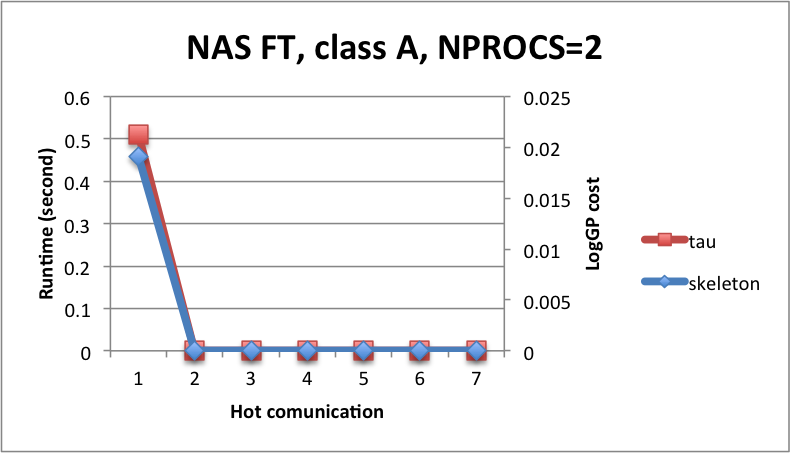
\includegraphics[width=.9\textwidth]{fig/blues/ft_A_2_model.png}
%\caption{Communication on 2 nodes}
%\label{fig:model:ft:A:2}
%\end{subfigure}
%\begin{subfigure}{.48\textwidth}
%\centering
%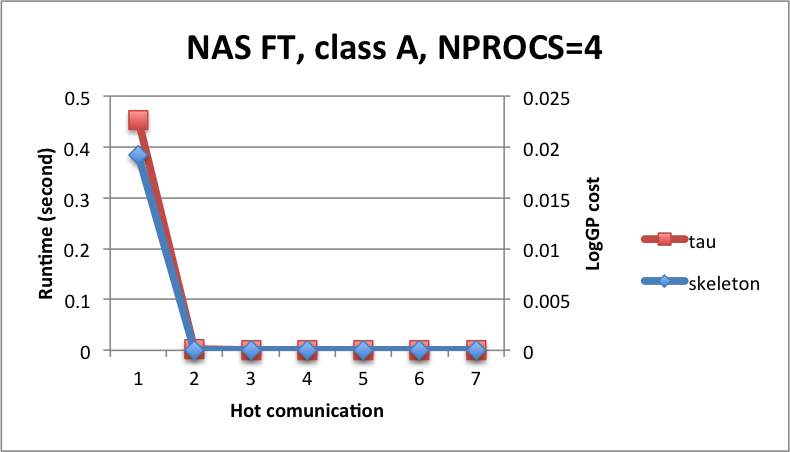
\includegraphics[width=.9\textwidth]{fig/blues/ft_A_4_model.png}
%\caption{Communication on 4 nodes}
%\label{fig:model:ft:A:4}
%\end{subfigure}
%\caption{Profiled runtime and modeled cost of NAS FT with small input (A) on x86 cluster}
%\label{fig:model:ft:A}
%}%\scriptsize
%\end{figure}

\begin{figure}
{\scriptsize
\begin{subfigure}{.48\textwidth}
\centering
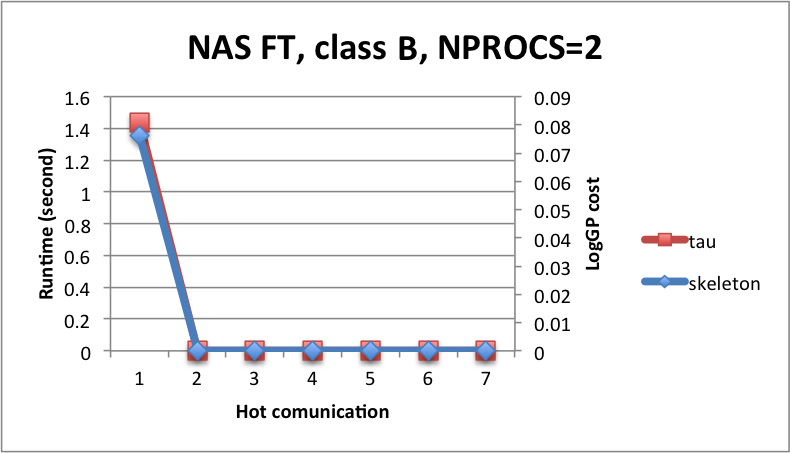
\includegraphics[width=.9\textwidth]{fig/blues/ft_B_2_model.png}
\caption{Communication on 2 nodes}
\label{fig:model:ft:B:2}
\end{subfigure}
\begin{subfigure}{.48\textwidth}
\centering
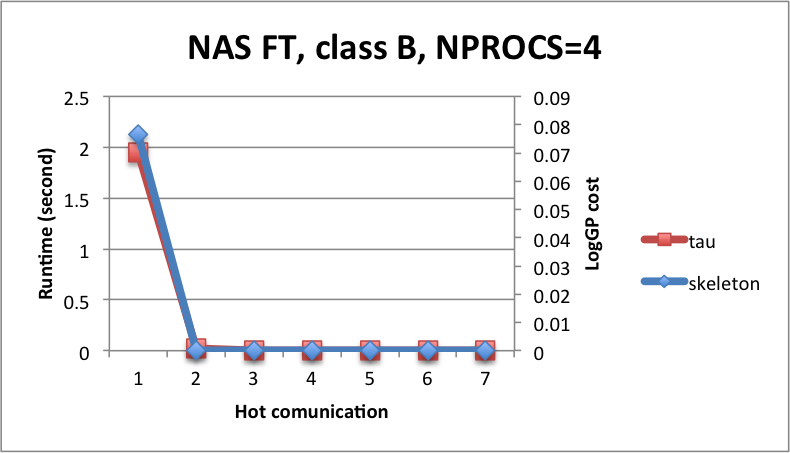
\includegraphics[width=.9\textwidth]{fig/blues/ft_B_4_model.png}
\caption{Communication on 4 nodes}
\label{fig::modelft:B:4}
\end{subfigure}
\caption{Profiled runtime and modeled cost of NAS FT with middle-sized input (B) on x86 cluster}
\label{fig:model:ft:B}
}%\scriptsize
\end{figure}
%As shown in Figure~\ref{fig:model:ft:A} and Figure~\ref{fig:model:ft:B},
%  our modeling approach identified the same hot communication as the tau profiler.
%The most time consuming MPI call is MPI\_Alltoall, which takes more than 90\% of the total communication time.

% NPB class = B, NPROCS = 4
\begin{table}
\caption{
Differences between the projected hot-spot selection and
the measured hot-spot selection based on profiling with 80\% threshold for class B data on 4 nodes. Zero means
the set of $N$ hot spots equals the top $N$ hot spots.
}%\caption
%{\scriptsize
\begin{center}
\begin{tabular}{c|r|r|r|r|r|r|r|r}
\hline
&\multicolumn{7}{c}{Selected number of hot MPI communications}\\
        & 1 & 2 & 3 & 4 & 5 & 6 & 7 & 8 \\
\hline
FT      & 0 &   &   &   &   &   &   &   \\  % 1:MPI_Alltoall, 99%
IS      & 0 & 0 &   &   &   &   &   &   \\  % 1:MPI_Alltoallv = 3.494, MPI_Allreduce = 1.279
CG      & 0 &   &   &   &   &   &   &   \\  % 1:MPI_Send 6,383, 2:MPI_Irecv
LU      & 0 & 1 & 2 & 2 & 1 & 1 & 0 & 0 \\  % MPI_Send
MG      & 1 & 1 & 0 & 1 & 1 & 0 &   &   \\  % MPI_Send
\hline
\hline
\end{tabular}
\end{center}
%}%\scriptsize
\label{tab:npb:hot}
\end{table}

%\begin{figure}
%{\scriptsize
%\centering
%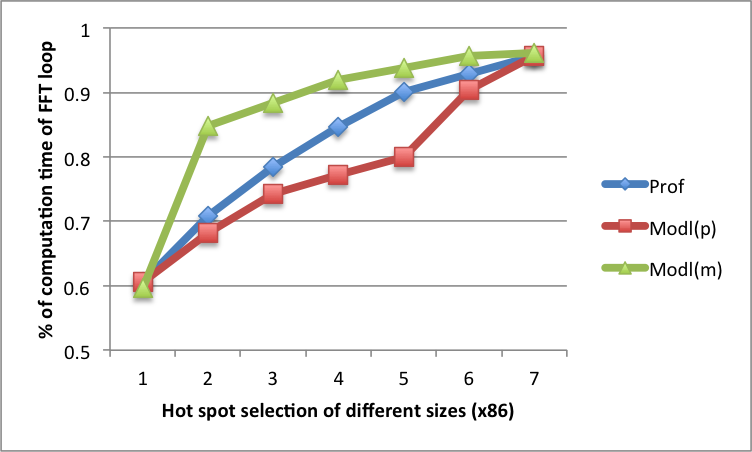
\includegraphics[width=.48\textwidth]{fig/blues/ft_B_4_hotspot.png}
%\caption{
%Profiled and modeled computation time of NAS FT's overlap region (the FFT loop) with middle-sized input (B) on 4 x86 nodes.
%{\tt Prof} and {\tt Modl} refer to the hot spot
%selections resulted from BG/Q profiling and performance modeling.
%{\tt Modl(p)} and {\tt Modl(m)} show the projected and measured
%runtime coverage on x86 cluster using the model-projected hot spots, respectively.
%}%\caption
%\label{fig:hot:ft}
%}%\scriptsize
%\end{figure}

%\begin{table}
%%{\scriptsize
%\begin{center}
%\begin{tabular}{c|r r r r r r r}
%\hline
%&\multicolumn{7}{c}{Sizes of local hot spot selections}\\
%        & 1 & 2 & 3 & 4 & 5 & 6 & 7 \\
%\hline
%FT      & 0 & 1 & 1 & 1 & 2 & 1 & 0 \\
%\hline
%\hline
%\end{tabular}
%\end{center}
%%}%\scriptsize
%\caption{
%\IPDPS{Differences between the projected hot spot selection and
%the measured hot spot selection based on profiling. Zero means
%the set of $N$ hot spots equals the top $N$ hot spots.
%%Q.{\tt Modl} and X.{\tt Modl} refer to hot spot selections for
%%BG/Q and Xeon based on our modeling, respectively.
%%Q.{\tt Xeon} refers to hot spot selection for BG/Q based on Xeon profiling.
%%X.{\tt BG/Q} refers to hot spot selection for Xeon based on BG/Q profiling.
%}
%}%\caption
%\label{tab:hot:ft}
%\end{table}

\subsection{Impact of Optimizations}
%\begin{figure}
%{\scriptsize
%\centering
%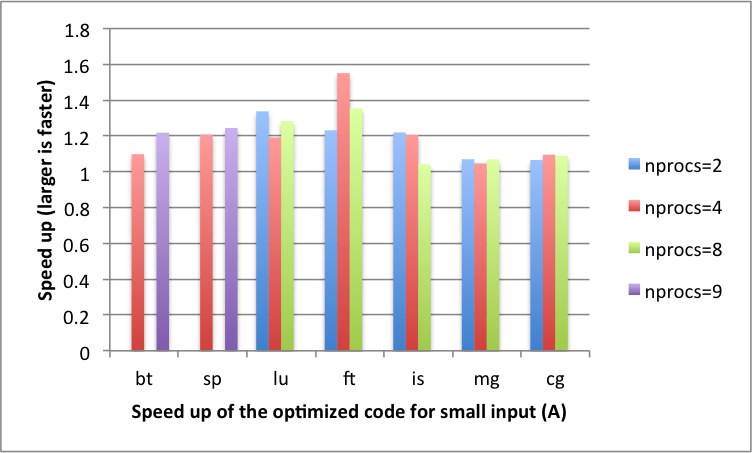
\includegraphics[width=.8\textwidth]{fig/disco/npb_disco_A.png}
%\caption{Speed up of NPB with input A class}
%\label{fig:npb:A}
%}%\scriptsize
%\end{figure}
\begin{figure}
{\scriptsize
\centering
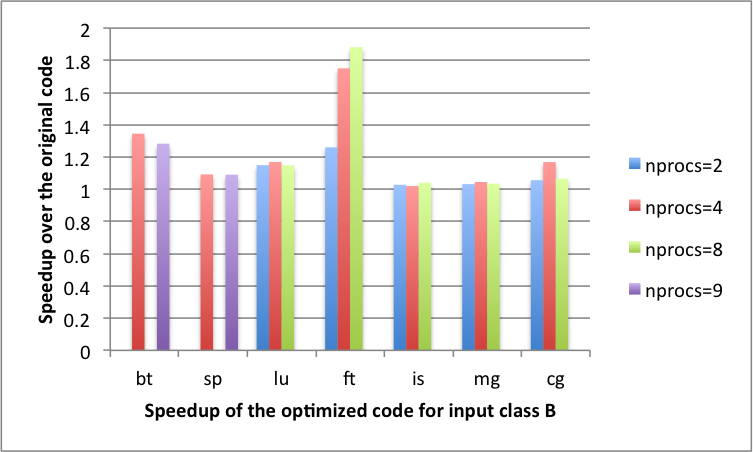
\includegraphics[width=.48\textwidth]{fig/blues/npb_blues_B.png}
\caption{Optimization speedups on the InfiniBand cluster.}
\label{fig:npb:x86}
}%\scriptsize
\end{figure}
\begin{figure}
{\scriptsize
\centering
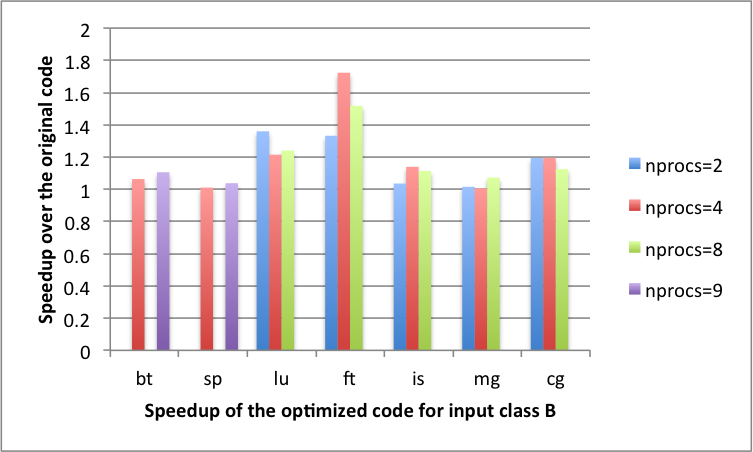
\includegraphics[width=.48\textwidth]{fig/disco/npb_disco_B.png}
\caption{Optimization speedups on the Ethernet cluster.}
\label{fig:npb:x64}
}
\end{figure}
%\begin{figure}
%{\scriptsize
%\centering
%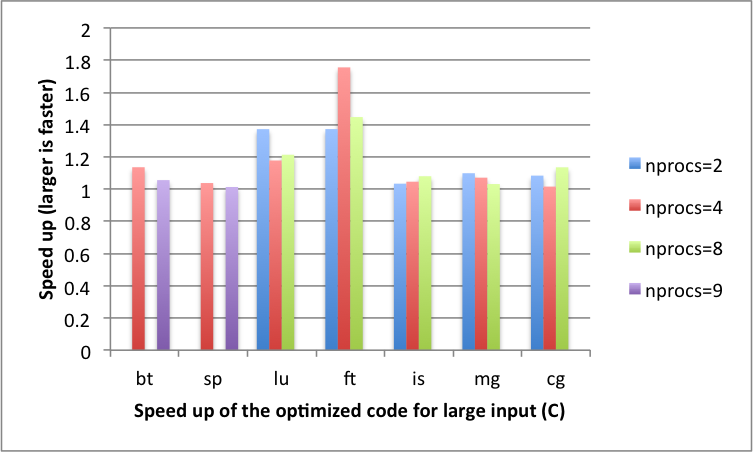
\includegraphics[width=.8\textwidth]{fig/disco/npb_disco_C.png}
%\caption{Speed up of NPB with input C class}
%\label{fig:npb:C}
%}%\scriptsize
%\end{figure}


Figures~\ref{fig:npb:x86} and \ref{fig:npb:x64}
show the speedups we attained by enabling better computation-communication overlapping for the NPB applications.
In particular, for each benchmark, the performance of the original application and the optimized code is measured by using input class B on 2, 4, 8, and 9 nodes,  with one MPI process bound to each node, 
with the exception of NAS BT and SP, which require the number of processes to be a multiple of 3 and so are configured to run on 3 and 9 nodes only.
The overall elapsed time of each application is measured by using NPB's built-in timer, which reports the elapsed time of multiple iterations with the exclusion of the initialization time.


Among all the NPB applications, FT and IS are the only benchmarks that use {\em alltoall} collectives as the main communication operation; the other benchmarks mostly use point-to-point send/receives.
Our optimization attained 3--88\% speedup for all applications.
The maximum 88\% performance improvement is observed with the NAS FT benchmark, which uses a time-consuming $MPI\_Alltoall$ operation, enclosed inside the outermost loop of the application,  to exchange a large amount of data.
The lowest speedup (3\%) is observed with NAS MG, which does not have sufficient local computation in the surrounding loop of the MPI communication to overlap with communication. \todo { I think we need to discuss more the difference between using the two different platforms}

%Another application NAS IS has the similar structure whose main loop is also the same as its communication loop.
%However, its most time-consuming communication is $MPI\_Alltoallv$ and the sizes of the communication data vary a lot at runtime.
%Depending on the input, the communication time of each $MPI\_Alltoallv$ call could be very short so that it is not able to hide the computation.
%As the result, our optimization is not able to achieve the same speedup as NAS FT.
%% 2. not single most consuming communication but multiple: lu, cg, bt, sp
%% MPI send/recv instead of alltoall.
%For NPB applications other than NAS FT and IS,
%  the majority of the communication time is spent on point-to-point send/receive instead of single alltoall collective calls.
%In these applications, there are communication calls that are not in loops, which we are not able to optimize.
%And the communication loops that we try to optimize are smaller than the main loop in these applications.
%As the result, not all computation is overlapped with the communication which result in less speedup.
% 3. Slowest mg, computation hot spot is out of communication loop
% The structure of MG is like this:
%   Loop
%     Loop -- the loop with interleaved computation/communication that we optimized
%       MainCommunication -- overlapped
%       VeryLittleComputation -- overlapped
%     MajorComputation -- not overlapped
%   Reduce -- final reduce outside of main loop that is also not overlapped


% EOF

%\subsubsection{NAS FT and IS}
%The most-time consuming communications are single all2all blocking collectives in the main loop,
%  and there is no overlapping of computation and communication at all in the original source code.
%Our optimization first converts blocking collectives to non-blocking versions,
%  and then reorders them to achieve overlap.
%Our optimization achieved the most speedup in NAS FT,
%  where the communication is $MPI\_Alltoall$
%  that always exchanges large amount of data.
%For NAS IS,
%   the most time-consuming communication IS is $MPI\_Alltoallv$ and the sizes of the data being communicated vary from less than 10 to as large as 30k.
%The communication time and computation time for IS is not always comparable.
%As the result, our optimization to overlap computation and communication saves more time for FT than for IS.
%
%\subsubsection{NAS BT and SP}
%The communications are done through non-blocking p2p send and receive in a group of $MPI\_Isend$, $MPI\_Irecv$, and $MPI\_Waitall$,
%  where the communications themselves in the same loop have already been overlapped.
%We first outline the consequent $MPI\_Isend$ and $MPI\_Irecv$ into the $Icomm(I)$ function and move $MPI\_Waitall$ into the $Wait(I)$ function,
%  and then reorder these communication with the nearby computation in the same loop to overlap them.
%Since the original communications are already non-blocking,
%  there is no need to convert the blocking communications to non-blocking versions.
%Comparing to FT and IS,
%  because the overlapped p2p communication exchanges less data and takes shorter time,
%  the overlap optimization achieves less speedup.
%
%\subsubsection{NAS MG, CG, and LU}
%The communications are done through pairs of blocking send and non-blocking receive ($MPI\_Send$, $MPI\_Irecv$, and $MPI\_Wait$),
%  but there is no overlapping of computation and communication in the original implementation.
%In our optimization, we first convert $MPI\_Send$ to $MPI\_Isend$ with $MPI\_Wait$,
%  then outline the $MPI\_Isend$ and $MPI\_Irecv$ into the $Icomm(I)$ function and their $MPI\_Wait$ into the $Wait(I)$ function,
%  and at last reorder these communication with the nearby computation in the same loop to achieve overlap.
%The structures of the optimized communication loops in CG and MG are similar,
%  where the communication takes much more time than the computation in the same loop.
%% jichi: MG and CG are like this
%% Loop:
%%   some computation -- not overlapped
%%   Loop:
%%     some computation  -- overlapped
%%     hot communication
%%   some computation -- not overlapped
%Additionally, some computation hot spots are not in the communication loop and not overlapped as the result,
%  which limit our overall speedup of our CCO optimization.
%In comparison, LU achieves better speedup,
%  where the hot communication takes less time than the computation in the same loop
%  and hence the communication latency can be fully hidden in the computation time.

%\subsubsection{Load balance}
%
%\begin{figure}
%{\scriptsize
%\centering
%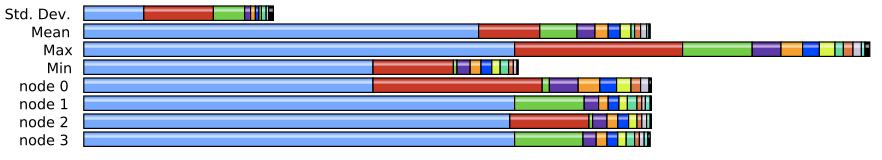
\includegraphics[width=.9\textwidth]{fig/blues/ft_B_4_tau.png}
%\caption{Runtime of NAS FT with middle-sized input (B) on 4 x86 nodes}
%\label{fig:opt:ft:B}
%}%\scriptsize
%\end{figure}
%
%\begin{figure}
%{\scriptsize
%\centering
%\includegraphics[width=.9\textwidth]{fig/blues/is_B_4_tau.png}
%\caption{Runtime of NAS IS with middle-sized input (B) on 4 x86 nodes}
%\label{fig:opt:ft:B}
%}%\scriptsize
%\end{figure}
%
%\begin{figure}
%{\scriptsize
%\centering
%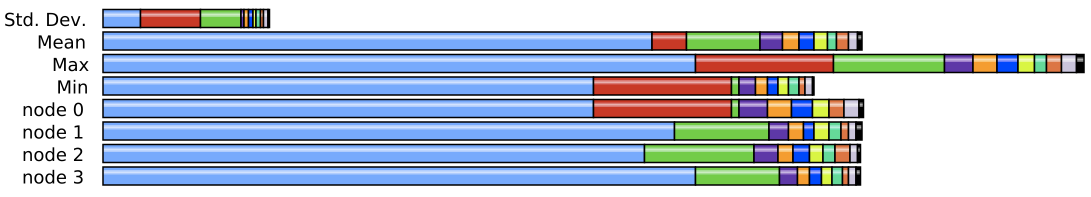
\includegraphics[width=.9\textwidth]{fig/disco/ft_B_4_tau.png}
%\caption{Runtime of NAS FT with middle-sized input (B) on 4 x86\_64 nodes}
%\label{fig:opt:ft:B}
%}%\scriptsize
%\end{figure}
%
%\begin{figure}
%{\scriptsize
%\centering
%\includegraphics[width=.9\textwidth]{fig/disco/is_B_4_tau.png}
%\caption{Runtime of NAS IS with middle-sized input (B) on 4 x86\_64 nodes}
%\label{fig:opt:ft:B}
%}%\scriptsize
%\end{figure}
%\subsection{Insertion of MPI\_Test}
%\begin{figure}
%\centering
%{\scriptsize
%\begin{verbatim}
%Loop J = 1 ... M
%  MPI_Ialltoall
%  Loop I = 1 ... N
%    If I % Freq == 0
%      MPI_Test
%    nanosleep
%  MPI_Wait
%\end{verbatim}
%\caption{The micro benchmark used to test distribution of MPI\_Test}
%\label{fig:cco_test}
%}%\scriptsize
%\end{figure}
%\begin{table}
%{\scriptsize\centering
%\begin{tabular}{|l|l|l|} \hline
%Distribution    & Time (sec) & Descriptions \\
%\hline
%orig            & 5.424621  & original benchmark without overlapping \\
%orig-comm       & 2.224972  & total communication time of the original code \\
%orig-comp       & 3.2       & total computation time of the original code \\
%5-test          & 3.56385   & evenly insert 5 MPI\_Test \\
%8-test          & 3.229617  & evenly insert 8 MPI\_Test \\
%10-test         & 3.15611   & evenly insert 10 MPI\_Test \\
%16-test         & 3.249664  & evenly insert 16 MPI\_Test \\
%100-test        & 3.590359  & evenly insert 100 MPI\_Test \\
%1000-test       & 17.265191 & evenly insert 1000 MPI\_Test \\
%unevel1-10-test & 3.939304  & unevenly first insert 8 slow and 2 fast MPI\_Test \\
%unevel2-10-test & 3.624152  & unevenly first insert 2 slow and 8 fast MPI\_Test \\
%\hline
%\end{tabular}
%}%\scriptsize
%\caption{Micro benchmark of overlapped MPI\_Alltoall}
%\label{tab:mpitest}
%\end{table}
%\begin{figure}
%{\scriptsize
%\centering
%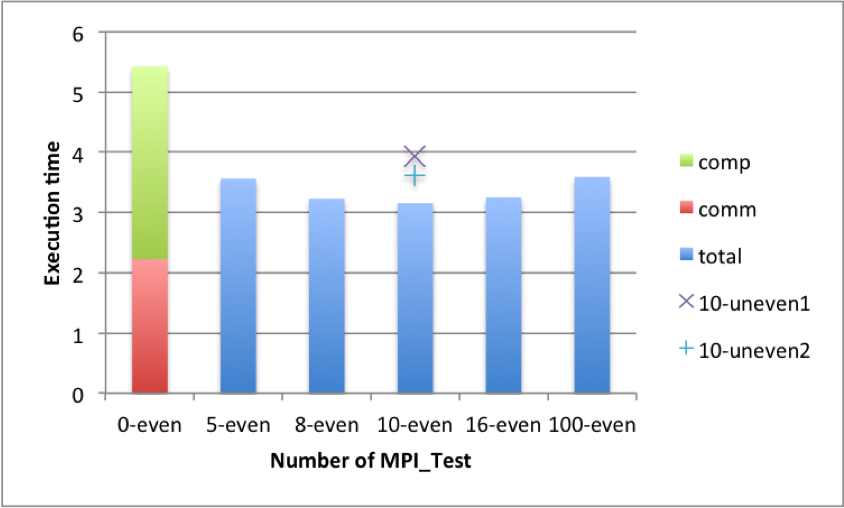
\includegraphics[width=.48\textwidth]{fig/mpitest.png}
%\caption{Micro benchmark of overlapped MPI\_Alltoall}
%\label{fig:exp:mpitest}
%}%\scriptsize
%\end{figure}
%To evaluate the impact of MPI\_Test distribution to the overlapping of computation and communication,
%  we designed a micro benchmark as shown in Figure~\ref{fig:exp:mpitest}.
%It contains a single loop of MPI\_Alltoall,
%  and a loop of computation emulated using $nanosleep()$.
%The execution time is shown in Figure~\ref{fig:exp:mpitest} and Table~\ref{tab:mpitest}.
%We tried different numbers of MPI\_Test when even distributed,
%  which shows the 10 MPI\_Test configuration has the best performance,
%  and the execution is monotoned increasing when the number of MPI\_Test is increasing or decreasing.
%This implies the best MPI\_Test frequency can be tuned through binary search.
%Given 10 MPI\_Test,
%  we also tried non-evenly distributed cases of \texttt{unevel1-10-test} and \texttt{uneven2-10-test},
%  where the sleep time between 2 MPI\_Test is will be 4 times slower than the sleep time between the other 8 MPI\_Test.
%Both the non-evenly distribution cases are slower than the evenly distributed MPI\_Test.
%NAS DT (Data Traffic) and EP (Embarrassingly Parallel) are excluded, which cannot benefit from our optimization approach.

\section{Related Work}
\label{sec-related}

Existing work on enhancing the efficiency of MPI applications has 
focused mostly on communication mechanisms underlying the many 
MPI operations, for example, alternative protocols for point-to-point
communications~\cite{brightwell:eurompi03,denis:eurompi11}, collective
operations~\cite{traff:eurompi14:ocd,traff:eurompi14:mcd,graham:eurompi08,mittal:ppopp12},
remote direct memory access
(RDMA)~\cite{liu:ics03,woodall:eurompi06,hatanaka:eurompi13}, load
balancing~\cite{nian:niss09,kale:eurompi14}, and the
elimination of redundant communications through software caching and
the exploitation of data
locality~\cite{buntinas:icpp09,isujita:eurompi14,ozog:ics13}.  In
contrast, our work focuses on application-level performance
enhancement by enabling automated overlapping of MPI communications
with independent local computations.

Iancu et al.~\cite{iancu:ppopp07} tried to automatically determine
message sizes and schedules for MPI communications through an
analytical model of system scale and load to avoid network congestion.
Danalis et al.~\cite{danalis:ics09} investigated compiler
optimizations to potentially automate the overlapping of 
computations and MPI communications, by formulating the side effects of key MPI operations so that
an MPI-aware compiler can automatically assess the safety of several
optimizations, which were then manually applied in their paper.
Various patterns of computation-communication overlapping and
automated optimization schemes have also been
discussed~\cite{danalis:sc05,fishgold:ipdps06}.  Our work also aims to automate the optimization
of MPI applications, by automatically determining the safety of reordering optimizations through compiler 
dependence analysis and the profitability of optimizations from 
analytical performance modeling. Our work particularly focuses on automatically enabling 
a special form of loop-based
communication-computation overlapping in scientific applications. 

%To reason about the profitability of optimizing MPI applications,
Sancho et al.~\cite{sancho:sc06} combined empirical tuning with
networking models to quantify the potential benefit of overlapping
communication and computation in large-scale scientific applications.
Potluri et al.~\cite{potluri:ics10} empirically quantified the
overlapping of MPI-2 operations in a seismic modeling application.  Hu
et al.~\cite{hu:npc08,song:ppopp14} identified the consumer-producer
model from the control flow graph of the application to guide
optimization decisions for overlapping Alltoall communication in a 3-D
FFT.  Didelot et al.~\cite{didelot:imc14,didelot:eurompi12} developed
a message progression model based on collaborative polling that allows
an efficient auto-adaptive overlapping of communication phases with
computation.  In this paper, we predicted the most time-consuming
code paths that contain MPI communications to
optimize, using existing analytical models of
communications~\cite{loggp}.

Preissl et al.~\cite{preissl:tms10} summarized common communication
patterns in MPI applications to enable automated optimization.
Pellegrini et al.~\cite{pellegrini:eurompi12} proposed an exact
dependence analysis approach for increasing the overlapping of
computation and communication.  Subotic et al.~\cite{subotic:hipeac08}
speculatively extracted runtime data-flow to understand the dynamic
dependence of the application.  Aananthakrishnan et
al.~\cite{aananthakrishnan:ics13} used a hybrid static and runtime
data-flow analysis of MPI programs.  We also use dependence analysis
to determine the correctness of optimization, enhanced with additional
knowledge from developers about their applications.

In order to find the optimal placement of nonblocking MPI operations
within the computation control flow, accurate modeling of the
underlying computation and communication is
required~\cite{brightwell:ics04}.  Hoefler et
al.~\cite{hoefler:icppw05} presented an analytical approach to model
MPI barriers.  Ino et al.~\cite{ino:ppopp2001} presented a parallel
computational model for synchronization analysis in MPI.  Martinez et
al.~\cite{martinez:ipdps09} developed an analytical model extending
LogGP~\cite{loggp} for accurate estimation of individual MPI
communication.  Moritz and Frank~\cite{moritz:tpds01} modeled network
contention in MPI applications.  In our optimization, we first
reposition each pair of local computation and nonblocking
communication as far apart as safety allows across different loop
iterations and then insert MPI\_Test with empirically tuned frequencies
into the local computation to ensure proper progress of the
nonblocking communication.

\section{Conclusion}
\label{sec-concl}

This paper presents a systematic approach to automate the overlapping
of communications with independent computations in large MPI
applications, thereby enhancing their performance portability.  Our
optimization workflow starts with analytical performance modeling of
the overall application execution flow to identify long-lasting MPI
communications to overlap. Next, we conduct automated safety
and profitability analysis (with optional developer assistance) to find optimization opportunities. We
complete the optimization by manually applying the necessary
transformations in a systematic fashion that can be potentially
automated.  We applied our approach to optimize 7 NAS NPB applications
on both a high-speed and a slow network-connected cluster
environment. We achieved 3--88\% speedup on both platforms.


\REMOVE{
\section*{Acknowledgment}
The research is partially funded by the National Science Foundation of USA
under Grants 1261778, 1261811, and 1261.
This research used resources of the Argonne Leadership Computing
Facility at Argonne National Laboratory, which is supported by the
Office of Science of the U.S. Department of Energy under contract
DE-AC02-06CH11357.
}


\bibliographystyle{plain}
\bibliography{bib/refs,bib/hotpath,bib/qing,bib/mpi,bib/jichi,bib/bench,bib/cco}
%\bibliography{venkat, jmeng, kk}

%\clearpage
\REMOVE{
\framebox{
\parbox{3.2in}{
The submitted manuscript has been created by UChicago Argonne, LLC, Operator of Argonne National Laboratory (``Argonne"). Argonne, a U.S. Department of Energy Office of Science laboratory, is operated under Contract No. DE-AC02-06CH11357. The U.S. Government retains for itself, and others acting on its behalf, a paid-up nonexclusive, irrevocable worldwide license in said article to reproduce, prepare derivative works, distribute copies to the public, and perform publicly and display publicly, by or on behalf of the Government.
}
}
}

% that's all folks
\end{document}

% EOF
